% Options for packages loaded elsewhere
\PassOptionsToPackage{unicode}{hyperref}
\PassOptionsToPackage{hyphens}{url}
\PassOptionsToPackage{dvipsnames,svgnames,x11names}{xcolor}
%
\documentclass[
  a4paper,
]{article}
\usepackage{amsmath,amssymb}
\usepackage{iftex}
\ifPDFTeX
  \usepackage[T1]{fontenc}
  \usepackage[utf8]{inputenc}
  \usepackage{textcomp} % provide euro and other symbols
\else % if luatex or xetex
  \usepackage{unicode-math} % this also loads fontspec
  \defaultfontfeatures{Scale=MatchLowercase}
  \defaultfontfeatures[\rmfamily]{Ligatures=TeX,Scale=1}
\fi
\usepackage{lmodern}
\ifPDFTeX\else
  % xetex/luatex font selection
\fi
% Use upquote if available, for straight quotes in verbatim environments
\IfFileExists{upquote.sty}{\usepackage{upquote}}{}
\IfFileExists{microtype.sty}{% use microtype if available
  \usepackage[]{microtype}
  \UseMicrotypeSet[protrusion]{basicmath} % disable protrusion for tt fonts
}{}
\makeatletter
\@ifundefined{KOMAClassName}{% if non-KOMA class
  \IfFileExists{parskip.sty}{%
    \usepackage{parskip}
  }{% else
    \setlength{\parindent}{0pt}
    \setlength{\parskip}{6pt plus 2pt minus 1pt}}
}{% if KOMA class
  \KOMAoptions{parskip=half}}
\makeatother
\usepackage{xcolor}
\usepackage[margin = 2cm]{geometry}
\usepackage{color}
\usepackage{fancyvrb}
\newcommand{\VerbBar}{|}
\newcommand{\VERB}{\Verb[commandchars=\\\{\}]}
\DefineVerbatimEnvironment{Highlighting}{Verbatim}{commandchars=\\\{\}}
% Add ',fontsize=\small' for more characters per line
\usepackage{framed}
\definecolor{shadecolor}{RGB}{248,248,248}
\newenvironment{Shaded}{\begin{snugshade}}{\end{snugshade}}
\newcommand{\AlertTok}[1]{\textcolor[rgb]{0.94,0.16,0.16}{#1}}
\newcommand{\AnnotationTok}[1]{\textcolor[rgb]{0.56,0.35,0.01}{\textbf{\textit{#1}}}}
\newcommand{\AttributeTok}[1]{\textcolor[rgb]{0.13,0.29,0.53}{#1}}
\newcommand{\BaseNTok}[1]{\textcolor[rgb]{0.00,0.00,0.81}{#1}}
\newcommand{\BuiltInTok}[1]{#1}
\newcommand{\CharTok}[1]{\textcolor[rgb]{0.31,0.60,0.02}{#1}}
\newcommand{\CommentTok}[1]{\textcolor[rgb]{0.56,0.35,0.01}{\textit{#1}}}
\newcommand{\CommentVarTok}[1]{\textcolor[rgb]{0.56,0.35,0.01}{\textbf{\textit{#1}}}}
\newcommand{\ConstantTok}[1]{\textcolor[rgb]{0.56,0.35,0.01}{#1}}
\newcommand{\ControlFlowTok}[1]{\textcolor[rgb]{0.13,0.29,0.53}{\textbf{#1}}}
\newcommand{\DataTypeTok}[1]{\textcolor[rgb]{0.13,0.29,0.53}{#1}}
\newcommand{\DecValTok}[1]{\textcolor[rgb]{0.00,0.00,0.81}{#1}}
\newcommand{\DocumentationTok}[1]{\textcolor[rgb]{0.56,0.35,0.01}{\textbf{\textit{#1}}}}
\newcommand{\ErrorTok}[1]{\textcolor[rgb]{0.64,0.00,0.00}{\textbf{#1}}}
\newcommand{\ExtensionTok}[1]{#1}
\newcommand{\FloatTok}[1]{\textcolor[rgb]{0.00,0.00,0.81}{#1}}
\newcommand{\FunctionTok}[1]{\textcolor[rgb]{0.13,0.29,0.53}{\textbf{#1}}}
\newcommand{\ImportTok}[1]{#1}
\newcommand{\InformationTok}[1]{\textcolor[rgb]{0.56,0.35,0.01}{\textbf{\textit{#1}}}}
\newcommand{\KeywordTok}[1]{\textcolor[rgb]{0.13,0.29,0.53}{\textbf{#1}}}
\newcommand{\NormalTok}[1]{#1}
\newcommand{\OperatorTok}[1]{\textcolor[rgb]{0.81,0.36,0.00}{\textbf{#1}}}
\newcommand{\OtherTok}[1]{\textcolor[rgb]{0.56,0.35,0.01}{#1}}
\newcommand{\PreprocessorTok}[1]{\textcolor[rgb]{0.56,0.35,0.01}{\textit{#1}}}
\newcommand{\RegionMarkerTok}[1]{#1}
\newcommand{\SpecialCharTok}[1]{\textcolor[rgb]{0.81,0.36,0.00}{\textbf{#1}}}
\newcommand{\SpecialStringTok}[1]{\textcolor[rgb]{0.31,0.60,0.02}{#1}}
\newcommand{\StringTok}[1]{\textcolor[rgb]{0.31,0.60,0.02}{#1}}
\newcommand{\VariableTok}[1]{\textcolor[rgb]{0.00,0.00,0.00}{#1}}
\newcommand{\VerbatimStringTok}[1]{\textcolor[rgb]{0.31,0.60,0.02}{#1}}
\newcommand{\WarningTok}[1]{\textcolor[rgb]{0.56,0.35,0.01}{\textbf{\textit{#1}}}}
\usepackage{graphicx}
\makeatletter
\def\maxwidth{\ifdim\Gin@nat@width>\linewidth\linewidth\else\Gin@nat@width\fi}
\def\maxheight{\ifdim\Gin@nat@height>\textheight\textheight\else\Gin@nat@height\fi}
\makeatother
% Scale images if necessary, so that they will not overflow the page
% margins by default, and it is still possible to overwrite the defaults
% using explicit options in \includegraphics[width, height, ...]{}
\setkeys{Gin}{width=\maxwidth,height=\maxheight,keepaspectratio}
% Set default figure placement to htbp
\makeatletter
\def\fps@figure{htbp}
\makeatother
\setlength{\emergencystretch}{3em} % prevent overfull lines
\providecommand{\tightlist}{%
  \setlength{\itemsep}{0pt}\setlength{\parskip}{0pt}}
\setcounter{secnumdepth}{-\maxdimen} % remove section numbering
\usepackage{fvextra}
\DefineVerbatimEnvironment{Highlighting}{Verbatim}{breaklines,breaksymbolleft={},commandchars=\\\{\}}
\usepackage{tcolorbox}
\usepackage{graphicx}
\usepackage{booktabs}
\usepackage[default]{lato}
\ifLuaTeX
  \usepackage{selnolig}  % disable illegal ligatures
\fi
\usepackage[style=apa,]{biblatex}
\addbibresource{references.bib}
\usepackage{bookmark}
\IfFileExists{xurl.sty}{\usepackage{xurl}}{} % add URL line breaks if available
\urlstyle{same}
\hypersetup{
  pdftitle={Spatial Economics -- Assignment 2},
  pdfauthor={Max Heinze (h11742049@s.wu.ac.at); Jaime Miravet (h12235992@s.wu.ac.at); Jan Trimmel (h11809096@s.wu.ac.at)},
  colorlinks=true,
  linkcolor={Maroon},
  filecolor={Maroon},
  citecolor={DarkOrchid!65!black},
  urlcolor={DarkOrchid!65!black},
  pdfcreator={LaTeX via pandoc}}

\title{\textbf{Spatial Economics -- Assignment 2}}
\author{Max Heinze
(\href{mailto:h11742049@s.wu.ac.at}{\nolinkurl{h11742049@s.wu.ac.at}}) \and Jaime
Miravet
(\href{mailto:h12235992@s.wu.ac.at}{\nolinkurl{h12235992@s.wu.ac.at}}) \and Jan
Trimmel
(\href{mailto:h11809096@s.wu.ac.at}{\nolinkurl{h11809096@s.wu.ac.at}})}
\date{April 15, 2024}

\begin{document}
\maketitle

{
\hypersetup{linkcolor=}
\setcounter{tocdepth}{2}
\tableofcontents
}
\vspace{2em}

\begin{tcolorbox}
\centering \itshape The executable code that was used in compiling the assignment is available on GitHub at \url{https://github.com/maxmheinze/spatial}.
\end{tcolorbox}

\newpage

\section{Task A}\label{task-a}

\subsection{Productivity Growth Map}\label{productivity-growth-map}

First, we load both the datafile and shapefile, select the countries of
interest, and create the productivity growth rate variable.

\begin{Shaded}
\begin{Highlighting}[]
\NormalTok{pacman}\SpecialCharTok{::}\FunctionTok{p\_load}\NormalTok{(dplyr, ggplot2, sf, spdep, raster)}

\CommentTok{\# Load dataset and shapefile}
\FunctionTok{load}\NormalTok{(}\StringTok{"./assignment2/data/data1.rda"}\NormalTok{)}
\NormalTok{shp }\OtherTok{\textless{}{-}} \FunctionTok{st\_read}\NormalTok{(}\AttributeTok{dsn =} \StringTok{"./assignment2/data/EU27.shp"}\NormalTok{, }\AttributeTok{quiet =} \ConstantTok{TRUE}\NormalTok{)}

\CommentTok{\# Select variables of interest}
\NormalTok{vars }\OtherTok{\textless{}{-}} \FunctionTok{c}\NormalTok{(}\StringTok{"IDb"}\NormalTok{, }\StringTok{"pr80b"}\NormalTok{, }\StringTok{"pr103b"}\NormalTok{, }\StringTok{"lninv1b"}\NormalTok{, }\StringTok{"lndens.empb"}\NormalTok{)}
\NormalTok{data }\OtherTok{\textless{}{-}}\NormalTok{ data1[vars]}

\CommentTok{\# Create productivity growth variable for countries of interest}
\NormalTok{merged\_shp }\OtherTok{\textless{}{-}} \FunctionTok{left\_join}\NormalTok{(shp, data, }\AttributeTok{by =} \FunctionTok{c}\NormalTok{(}\AttributeTok{Id =} \StringTok{"IDb"}\NormalTok{))}
\NormalTok{countries }\OtherTok{\textless{}{-}} \FunctionTok{c}\NormalTok{(}\StringTok{"AT"}\NormalTok{, }\StringTok{"DE"}\NormalTok{, }\StringTok{"ES"}\NormalTok{, }\StringTok{"FR"}\NormalTok{, }\StringTok{"IT"}\NormalTok{, }\StringTok{"PT"}\NormalTok{)}
\NormalTok{df }\OtherTok{\textless{}{-}}\NormalTok{ merged\_shp[}\FunctionTok{grep}\NormalTok{(}\FunctionTok{paste}\NormalTok{(countries, }\AttributeTok{collapse =} \StringTok{"|"}\NormalTok{), merged\_shp}\SpecialCharTok{$}\NormalTok{Id), ]}
\NormalTok{df }\OtherTok{\textless{}{-}} \FunctionTok{na.omit}\NormalTok{(df)}
\NormalTok{df}\SpecialCharTok{$}\NormalTok{prgrowth }\OtherTok{\textless{}{-}}\NormalTok{ ((df}\SpecialCharTok{$}\NormalTok{pr103b }\SpecialCharTok{{-}}\NormalTok{ df}\SpecialCharTok{$}\NormalTok{pr80b)}\SpecialCharTok{/}\NormalTok{df}\SpecialCharTok{$}\NormalTok{pr80b) }\SpecialCharTok{*} \DecValTok{100}
\end{Highlighting}
\end{Shaded}

We create the productivty growth rate map:

\begin{Shaded}
\begin{Highlighting}[]
\CommentTok{\# Cut the productivity growth values into five segments to plot them}
\NormalTok{breaks }\OtherTok{\textless{}{-}} \FunctionTok{c}\NormalTok{(}\SpecialCharTok{{-}}\DecValTok{20}\NormalTok{, }\SpecialCharTok{{-}}\DecValTok{10}\NormalTok{, }\DecValTok{0}\NormalTok{, }\DecValTok{15}\NormalTok{, }\DecValTok{30}\NormalTok{, }\DecValTok{50}\NormalTok{)}
\NormalTok{labels }\OtherTok{\textless{}{-}} \FunctionTok{c}\NormalTok{(}\StringTok{"({-}20,{-}10)"}\NormalTok{, }\StringTok{"({-}10,0)"}\NormalTok{, }\StringTok{"(0,15)"}\NormalTok{, }\StringTok{"(15,30)"}\NormalTok{, }\StringTok{"(30,50)"}\NormalTok{)}
\NormalTok{df}\SpecialCharTok{$}\NormalTok{prgrowth\_bins }\OtherTok{\textless{}{-}} \FunctionTok{cut}\NormalTok{(df}\SpecialCharTok{$}\NormalTok{prgrowth, }\AttributeTok{breaks =}\NormalTok{ breaks, }\AttributeTok{labels =}\NormalTok{ labels)}

\CommentTok{\# Visualization of productivity growth rate}
\NormalTok{bin\_colors }\OtherTok{\textless{}{-}} \FunctionTok{c}\NormalTok{(}\StringTok{"lightyellow"}\NormalTok{, }\StringTok{"yellow"}\NormalTok{, }\StringTok{"orange"}\NormalTok{, }\StringTok{"red"}\NormalTok{, }\StringTok{"brown"}\NormalTok{)}
\FunctionTok{ggplot}\NormalTok{() }\SpecialCharTok{+} \FunctionTok{geom\_sf}\NormalTok{(}\AttributeTok{data =}\NormalTok{ df, }\FunctionTok{aes}\NormalTok{(}\AttributeTok{fill =}\NormalTok{ prgrowth\_bins)) }\SpecialCharTok{+} \FunctionTok{scale\_fill\_manual}\NormalTok{(}\AttributeTok{name =} \StringTok{"\%"}\NormalTok{,}
    \AttributeTok{breaks =}\NormalTok{ labels, }\AttributeTok{values =}\NormalTok{ bin\_colors) }\SpecialCharTok{+} \FunctionTok{labs}\NormalTok{(}\AttributeTok{title =} \StringTok{"Productivity Growth Rate (1980{-}2003)"}\NormalTok{) }\SpecialCharTok{+}
    \FunctionTok{theme\_minimal}\NormalTok{()}
\end{Highlighting}
\end{Shaded}

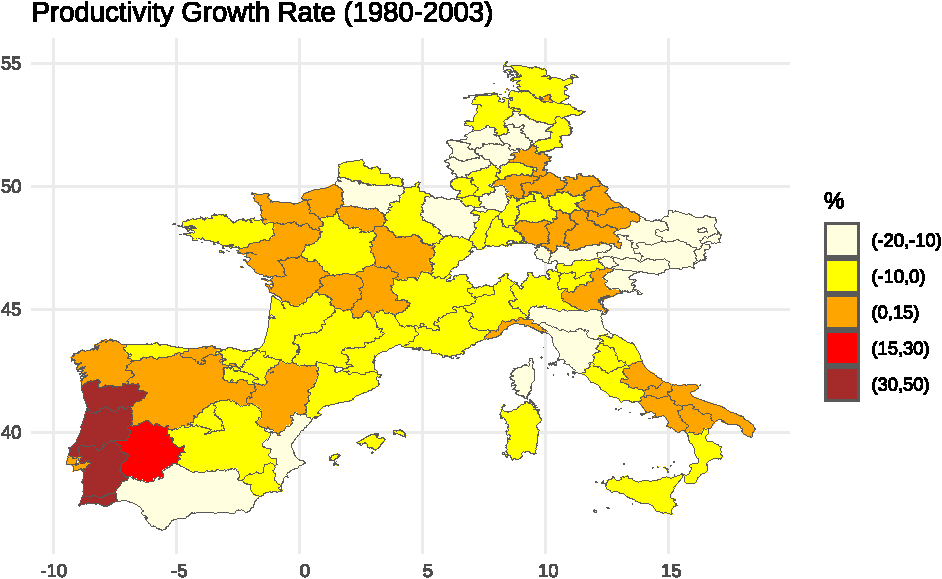
\includegraphics{assignment2_files/figure-latex/unnamed-chunk-2-1.pdf}

\subsection{Creating the weight
matrices}\label{creating-the-weight-matrices}

\subsubsection{(1) Distance threshold
matrix}\label{distance-threshold-matrix}

\begin{Shaded}
\begin{Highlighting}[]
\CommentTok{\# Create centroids of regions}
\NormalTok{centr }\OtherTok{\textless{}{-}} \FunctionTok{st\_centroid}\NormalTok{(df)}
\NormalTok{coord }\OtherTok{\textless{}{-}} \FunctionTok{st\_coordinates}\NormalTok{(centr)}
\NormalTok{dist }\OtherTok{\textless{}{-}} \FunctionTok{dnearneigh}\NormalTok{(coord, }\DecValTok{0}\NormalTok{, }\DecValTok{10000}\NormalTok{, }\AttributeTok{row.names =}\NormalTok{ df}\SpecialCharTok{$}\NormalTok{Id)}

\CommentTok{\# Minimum distance threshold so there are no disconnected regions}
\NormalTok{k1 }\OtherTok{\textless{}{-}} \FunctionTok{knearneigh}\NormalTok{(coord, }\AttributeTok{k =} \DecValTok{1}\NormalTok{)}
\NormalTok{k1 }\OtherTok{\textless{}{-}} \FunctionTok{knn2nb}\NormalTok{(k1)}
\NormalTok{min.max }\OtherTok{\textless{}{-}} \FunctionTok{max}\NormalTok{(}\FunctionTok{unlist}\NormalTok{(}\FunctionTok{nbdists}\NormalTok{(k1, }\AttributeTok{coords =}\NormalTok{ coord)))}
\NormalTok{min.max}
\end{Highlighting}
\end{Shaded}

\begin{verbatim}
## [1] 2.652709
\end{verbatim}

\begin{Shaded}
\begin{Highlighting}[]
\CommentTok{\# We use the obtained maximum value of the threshold}
\NormalTok{dist }\OtherTok{\textless{}{-}} \FunctionTok{dnearneigh}\NormalTok{(coord, }\DecValTok{0}\NormalTok{, min.max, }\AttributeTok{row.names =}\NormalTok{ df}\SpecialCharTok{$}\NormalTok{Id)}

\CommentTok{\# With this new distance threshold, each region has an average of 8.3 links.}

\NormalTok{w1 }\OtherTok{\textless{}{-}} \FunctionTok{nb2mat}\NormalTok{(dist, }\AttributeTok{style =} \StringTok{"W"}\NormalTok{)}
\end{Highlighting}
\end{Shaded}

It appears that setting a large maximum value in the distance threshold
yields too many links per region. Therefore, we compute the minimum
value of the max. distance threshold so that no region is isolated. We
create a weight matrix in which each region has a positive value if its
kth neighbor is below the maximum distance threshold (around 2.65) and 0
if it is above.

\subsubsection{(2) Smooth distance-decay
matrix}\label{smooth-distance-decay-matrix}

We create a smooth distance-decay function so that the value decreases
as distance between regions increases by setting \(\delta\) = 0 in the
exponential function \(\exp[\delta d(i,j)]\). Then, we create a matrix
by transforming the distance matrix that contains the distances between
the centroids of the regions with the smooth distance-decay function

\begin{Shaded}
\begin{Highlighting}[]
\NormalTok{function0 }\OtherTok{\textless{}{-}} \ControlFlowTok{function}\NormalTok{(x) \{}
    \FunctionTok{exp}\NormalTok{(}\SpecialCharTok{{-}}\FloatTok{0.4} \SpecialCharTok{*}\NormalTok{ x)}
\NormalTok{\}}


\NormalTok{distance }\OtherTok{\textless{}{-}} \FunctionTok{st\_distance}\NormalTok{(centr)}
\NormalTok{g2 }\OtherTok{\textless{}{-}} \FunctionTok{matrix}\NormalTok{(}\ConstantTok{NA}\NormalTok{, }\AttributeTok{nrow =} \FunctionTok{nrow}\NormalTok{(distance), }\AttributeTok{ncol =} \FunctionTok{ncol}\NormalTok{(distance))}

\ControlFlowTok{for}\NormalTok{ (i }\ControlFlowTok{in} \FunctionTok{seq\_along}\NormalTok{(distance)) \{}
\NormalTok{    g2[i] }\OtherTok{\textless{}{-}} \FunctionTok{function0}\NormalTok{(distance[i])}
\NormalTok{\}}

\CommentTok{\# Finally, we row{-}normalize the matrix and set its diagonal to 0 to create a}
\CommentTok{\# weight matrix.}
\NormalTok{w2 }\OtherTok{\textless{}{-}}\NormalTok{ g2}\SpecialCharTok{/}\FunctionTok{rowSums}\NormalTok{(g2)}
\FunctionTok{diag}\NormalTok{(w2) }\OtherTok{\textless{}{-}} \DecValTok{0}
\end{Highlighting}
\end{Shaded}

\subsubsection{(3) Contiguity-based
matrix}\label{contiguity-based-matrix}

We construct a matrix such that in the row of each region each element
will be positive for contiguous neighbors and 0 otherwise.

\begin{Shaded}
\begin{Highlighting}[]
\NormalTok{contiguity }\OtherTok{\textless{}{-}} \FunctionTok{poly2nb}\NormalTok{(df, }\AttributeTok{row.names =}\NormalTok{ df}\SpecialCharTok{$}\NormalTok{Id, }\AttributeTok{queen =} \ConstantTok{TRUE}\NormalTok{)}

\NormalTok{w3 }\OtherTok{\textless{}{-}} \FunctionTok{nb2mat}\NormalTok{(contiguity, }\AttributeTok{style =} \StringTok{"W"}\NormalTok{, }\AttributeTok{zero.policy =} \ConstantTok{TRUE}\NormalTok{)}
\CommentTok{\# zero.policy is set to TRUE since there are regions with no contiguous}
\CommentTok{\# neighbors}
\end{Highlighting}
\end{Shaded}

\subsection{Comparing the matrices}\label{comparing-the-matrices}

First, we can compute the sparsity of each matrix (proportion of zero
elements).

\begin{Shaded}
\begin{Highlighting}[]
\NormalTok{sp1 }\OtherTok{\textless{}{-}} \FunctionTok{sum}\NormalTok{(w1 }\SpecialCharTok{==} \DecValTok{0}\NormalTok{)}\SpecialCharTok{/}\FunctionTok{length}\NormalTok{(w1)}
\NormalTok{sp2 }\OtherTok{\textless{}{-}} \FunctionTok{sum}\NormalTok{(w2 }\SpecialCharTok{==} \DecValTok{0}\NormalTok{)}\SpecialCharTok{/}\FunctionTok{length}\NormalTok{(w2)}
\NormalTok{sp3 }\OtherTok{\textless{}{-}} \FunctionTok{sum}\NormalTok{(w3 }\SpecialCharTok{==} \DecValTok{0}\NormalTok{)}\SpecialCharTok{/}\FunctionTok{length}\NormalTok{(w3)}
\NormalTok{sparsity }\OtherTok{\textless{}{-}} \FunctionTok{c}\NormalTok{(sp1, sp2, sp3)}
\FunctionTok{names}\NormalTok{(sparsity) }\OtherTok{\textless{}{-}} \FunctionTok{c}\NormalTok{(}\StringTok{"W1"}\NormalTok{, }\StringTok{"W2"}\NormalTok{, }\StringTok{"W3"}\NormalTok{)}
\FunctionTok{print}\NormalTok{(sparsity)}
\end{Highlighting}
\end{Shaded}

\begin{verbatim}
##          W1          W2          W3 
## 0.918559713 0.009708738 0.958148742
\end{verbatim}

We observe that the elements of the matrices based on a distance
threshold and on contiguity are mostly zero.The matrix based on a smooth
distance-decay function has a much smaller proportion of zero elements.
On the one hand, given the small distance threshold imposed and the
large number of regions, it's not surprising that \(W_1\) and \(W_3\)
have mostly zero elements, representing no link with most neighbors. On
the other hand, since we use a decaying exponential function to
construct \(W_2\), even the regions that are furthest away from each
other have a positive value. Therefore, the only zero elements are
diagonal elements.

Then we compute their eigenvalues.

\begin{Shaded}
\begin{Highlighting}[]
\NormalTok{eigenw1 }\OtherTok{\textless{}{-}} \FunctionTok{eigen}\NormalTok{(w1)}\SpecialCharTok{$}\NormalTok{value}
\NormalTok{eigenw2 }\OtherTok{\textless{}{-}} \FunctionTok{eigen}\NormalTok{(w2)}\SpecialCharTok{$}\NormalTok{value}
\NormalTok{eigenw3 }\OtherTok{\textless{}{-}} \FunctionTok{eigen}\NormalTok{(w3)}\SpecialCharTok{$}\NormalTok{value}

\CommentTok{\# Since each matrix has 103 eigenvalues, we focus on the largest 5.}
\NormalTok{eigentop1 }\OtherTok{\textless{}{-}}\NormalTok{ eigenw1[}\DecValTok{1}\SpecialCharTok{:}\DecValTok{5}\NormalTok{]}
\NormalTok{eigentop2 }\OtherTok{\textless{}{-}}\NormalTok{ eigenw2[}\DecValTok{1}\SpecialCharTok{:}\DecValTok{5}\NormalTok{]}
\NormalTok{eigentop3 }\OtherTok{\textless{}{-}}\NormalTok{ eigenw3[}\DecValTok{1}\SpecialCharTok{:}\DecValTok{5}\NormalTok{]}

\NormalTok{eigenvalues }\OtherTok{\textless{}{-}} \FunctionTok{cbind}\NormalTok{(eigentop1, eigentop2, eigentop3)}
\FunctionTok{print}\NormalTok{(eigenvalues)}
\end{Highlighting}
\end{Shaded}

\begin{verbatim}
##      eigentop1 eigentop2 eigentop3
## [1,] 1.0000000 0.9136859 1.0000000
## [2,] 0.9909479 0.7346632 0.9877825
## [3,] 0.9560398 0.5670454 0.9787316
## [4,] 0.9471914 0.4869174 0.9596820
## [5,] 0.9090106 0.3743769 0.9451354
\end{verbatim}

We observe that the top 5 eigenvalues of \(W_1\) and \(W_3\) are larger
than those of \(W_2\). This shows there is stronger spatial
autocorrelation in \(W_1\) and \(W_3\). On the other hand, the
eigenvalues of \(W_1\) and \(W_3\) appear to decrease gradually, whereas
those of \(W_2\) decrease more rapidly. This indicates a faster decay in
spatial autocorrelation with distance in \(W_2\) compared to the other
two matrices.

Now, in order to analyze the matrices from a graph theory perspective,
we convert the weight matrices into adjacency (binary) matrices.

\begin{Shaded}
\begin{Highlighting}[]
\NormalTok{d1 }\OtherTok{\textless{}{-}} \FunctionTok{ifelse}\NormalTok{(w1 }\SpecialCharTok{\textgreater{}} \DecValTok{0}\NormalTok{, }\DecValTok{1}\NormalTok{, }\DecValTok{0}\NormalTok{)}
\NormalTok{d2 }\OtherTok{\textless{}{-}} \FunctionTok{ifelse}\NormalTok{(w2 }\SpecialCharTok{\textgreater{}} \DecValTok{0}\NormalTok{, }\DecValTok{1}\NormalTok{, }\DecValTok{0}\NormalTok{)}
\NormalTok{d3 }\OtherTok{\textless{}{-}} \FunctionTok{ifelse}\NormalTok{(w3 }\SpecialCharTok{\textgreater{}} \DecValTok{0}\NormalTok{, }\DecValTok{1}\NormalTok{, }\DecValTok{0}\NormalTok{)}
\end{Highlighting}
\end{Shaded}

Once we have adjacency matrices, we can compute their degree
distribution. Note that since \(W_2\) has no zero off-diagonal elements,
every region is connected to each other, so there is no point on
computing the degree distribution of \(D_2\).

\begin{Shaded}
\begin{Highlighting}[]
\NormalTok{node\_degrees1 }\OtherTok{\textless{}{-}} \FunctionTok{rowSums}\NormalTok{(d1)}
\NormalTok{node\_degrees3 }\OtherTok{\textless{}{-}} \FunctionTok{rowSums}\NormalTok{(d3)}

\FunctionTok{hist}\NormalTok{(node\_degrees1, }\AttributeTok{main =} \StringTok{"Degree Distribution D1"}\NormalTok{, }\AttributeTok{xlab =} \StringTok{"Node Degree"}\NormalTok{, }\AttributeTok{ylab =} \StringTok{"Frequency"}\NormalTok{,}
    \AttributeTok{xlim =} \FunctionTok{c}\NormalTok{(}\DecValTok{0}\NormalTok{, }\DecValTok{25}\NormalTok{), }\AttributeTok{ylim =} \FunctionTok{c}\NormalTok{(}\DecValTok{0}\NormalTok{, }\DecValTok{25}\NormalTok{))}
\end{Highlighting}
\end{Shaded}

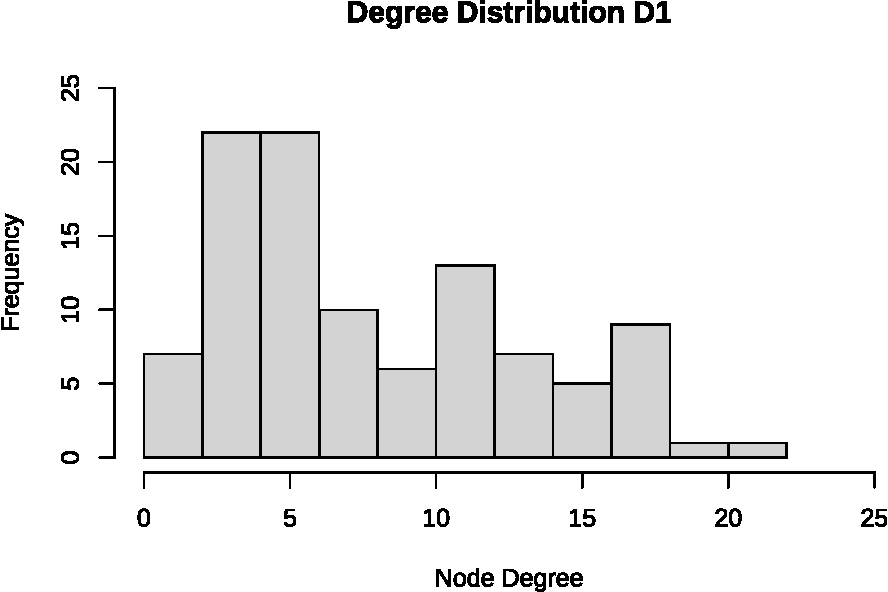
\includegraphics{assignment2_files/figure-latex/unnamed-chunk-9-1.pdf}

\begin{Shaded}
\begin{Highlighting}[]
\FunctionTok{hist}\NormalTok{(node\_degrees3, }\AttributeTok{main =} \StringTok{"Degree Distribution D3"}\NormalTok{, }\AttributeTok{xlab =} \StringTok{"Node Degree"}\NormalTok{, }\AttributeTok{ylab =} \StringTok{"Frequency"}\NormalTok{,}
    \AttributeTok{xlim =} \FunctionTok{c}\NormalTok{(}\DecValTok{0}\NormalTok{, }\DecValTok{15}\NormalTok{), }\AttributeTok{ylim =} \FunctionTok{c}\NormalTok{(}\DecValTok{0}\NormalTok{, }\DecValTok{25}\NormalTok{))}
\end{Highlighting}
\end{Shaded}

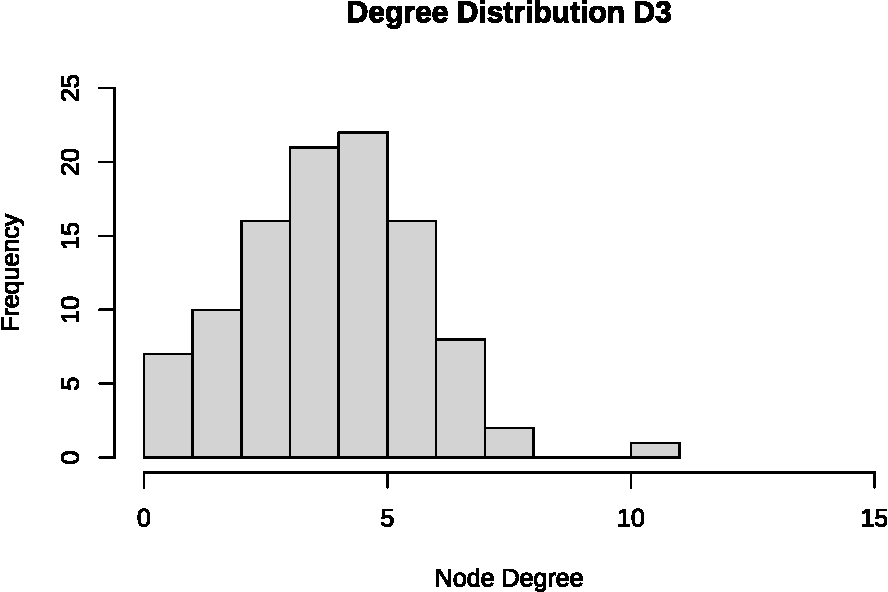
\includegraphics{assignment2_files/figure-latex/unnamed-chunk-9-2.pdf}

The adjacency matrix obtained when transforming \(W_1\), \(D_1\), shows
a degree distribution more spread and skewed to the right, whereas
\(D_3\) (transformed \(W_3\)) shows a more concentrated degree
distribution with hardly no skeewness.

\subsubsection{Plotting the matrices}\label{plotting-the-matrices}

\begin{Shaded}
\begin{Highlighting}[]
\NormalTok{v1 }\OtherTok{\textless{}{-}} \FunctionTok{raster}\NormalTok{(w1)}
\NormalTok{v2 }\OtherTok{\textless{}{-}} \FunctionTok{raster}\NormalTok{(w2)}
\NormalTok{v3 }\OtherTok{\textless{}{-}} \FunctionTok{raster}\NormalTok{(w3)}
\FunctionTok{plot}\NormalTok{(v1)}
\end{Highlighting}
\end{Shaded}

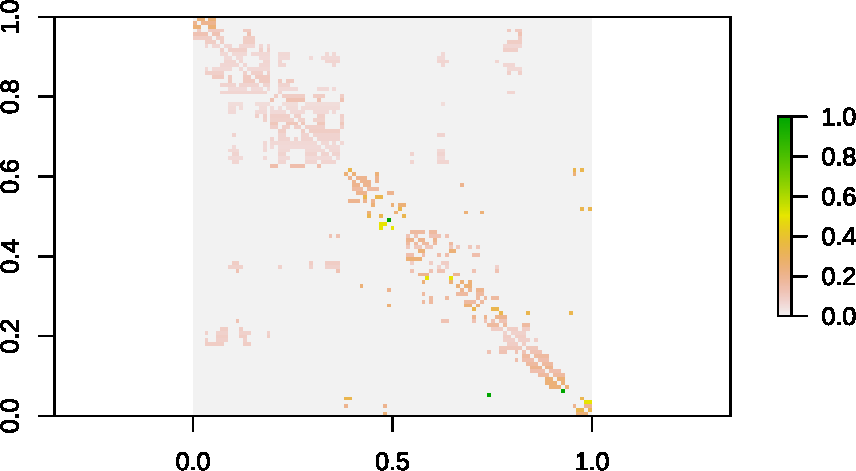
\includegraphics{assignment2_files/figure-latex/unnamed-chunk-10-1.pdf}

\begin{Shaded}
\begin{Highlighting}[]
\FunctionTok{plot}\NormalTok{(v2)}
\end{Highlighting}
\end{Shaded}

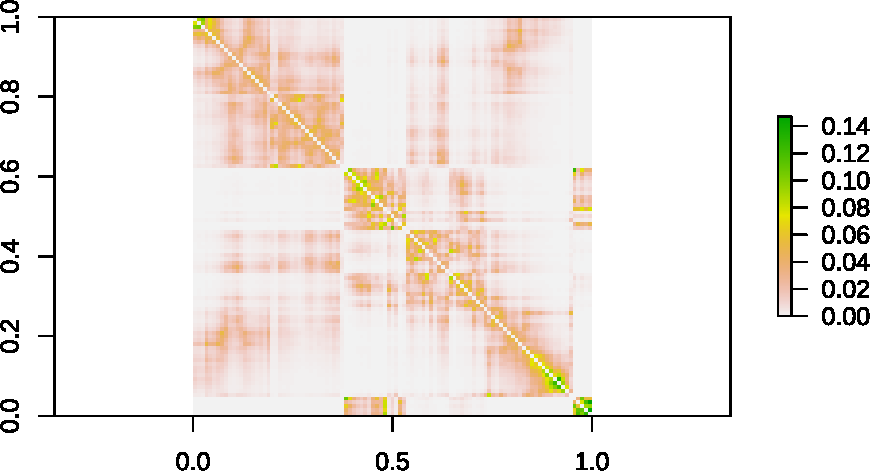
\includegraphics{assignment2_files/figure-latex/unnamed-chunk-10-2.pdf}

\begin{Shaded}
\begin{Highlighting}[]
\FunctionTok{plot}\NormalTok{(v3)}
\end{Highlighting}
\end{Shaded}

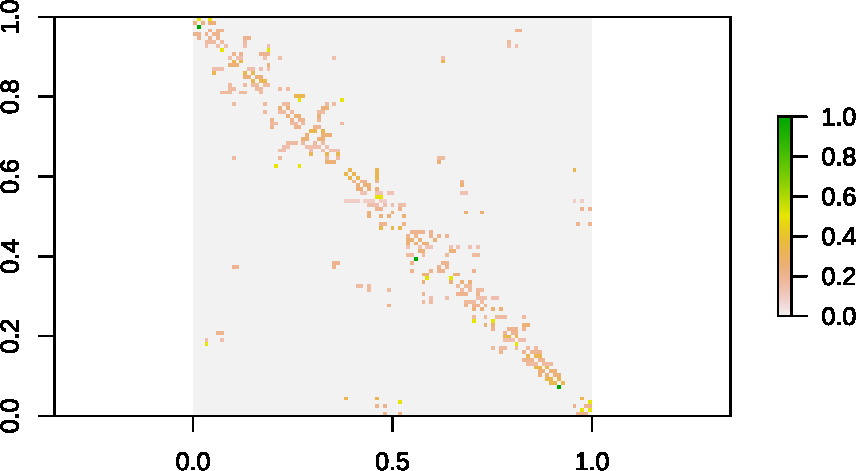
\includegraphics{assignment2_files/figure-latex/unnamed-chunk-10-3.pdf}

We observe that \(W_1\) and \(W_3\) represent a network there are less
connections between regions, but the existing links are stronger than
those of \(W_2\).The smooth distance-decay matrix \(W_2\), on the other
hand, represents a much more interconnected network, where each region
is connected to each other but the links are weaker on average.

\(W_2\) can help us visualize the clusters in the network. To do so, we
must take into account how the countries are ordered in the matrix. The
order (from first rows(columns) to last) is Austria, Germany, Spain,
France, Italy and Portugal. (This is because the region codes are
ordered alphabetically (AT, DE, ES, FR, IT, PT). Looking at \(W_2\) we
observe the biggest cluster is located among the Austrian and German
regions (top-left corner). Then, the smaller cluster in the middle
represents Spain. As we can see, Spanish regions have a almost
non-existing link with Austria and Germany, and their stronger links are
related to Portugal (middle of the bottom (or right) part). Then, in the
diagonal below Spain we see France. We can see how it is the country
with more connections to the rest of countries. Below in the diagonal we
observe the cluster formed by the Italian regions. We see that their
strongest foreign links are with Austrian regions. Finally, in the very
bottom-right corner we see Portugal. It is clear how Portuguese regions
are isolated from all countries except Spain.

\subsection{Computing a measure of spatial autocorrelation for
productivity
growth}\label{computing-a-measure-of-spatial-autocorrelation-for-productivity-growth}

To measure spatial autocorrelation, we will compute a Global Moran's I
statistic for each matrix.

\begin{Shaded}
\begin{Highlighting}[]
\CommentTok{\# (1) Distance threshold matrix}
\NormalTok{w1listw }\OtherTok{\textless{}{-}} \FunctionTok{mat2listw}\NormalTok{(w1, }\AttributeTok{style =} \StringTok{"W"}\NormalTok{)  }\CommentTok{\#We transform w1 into a listw so that moran.test() works}
\NormalTok{i1 }\OtherTok{\textless{}{-}} \FunctionTok{moran.test}\NormalTok{(df}\SpecialCharTok{$}\NormalTok{prgrowth, w1listw)}
\NormalTok{i1 }\OtherTok{\textless{}{-}}\NormalTok{ i1}\SpecialCharTok{$}\NormalTok{estimate[}\StringTok{"Moran I statistic"}\NormalTok{]}
\CommentTok{\# (2) Smooth distance{-}decay matrix}
\NormalTok{w2listw }\OtherTok{\textless{}{-}} \FunctionTok{mat2listw}\NormalTok{(w2, }\AttributeTok{style =} \StringTok{"W"}\NormalTok{)}
\NormalTok{i2 }\OtherTok{\textless{}{-}} \FunctionTok{moran.test}\NormalTok{(df}\SpecialCharTok{$}\NormalTok{prgrowth, w2listw)}
\NormalTok{i2 }\OtherTok{\textless{}{-}}\NormalTok{ i2}\SpecialCharTok{$}\NormalTok{estimate[}\StringTok{"Moran I statistic"}\NormalTok{]}
\CommentTok{\# (3) Contiguity matrix}
\NormalTok{w3listw }\OtherTok{\textless{}{-}} \FunctionTok{mat2listw}\NormalTok{(w3, }\AttributeTok{style =} \StringTok{"W"}\NormalTok{, }\AttributeTok{zero.policy =} \ConstantTok{TRUE}\NormalTok{)}
\NormalTok{i3 }\OtherTok{\textless{}{-}} \FunctionTok{moran.test}\NormalTok{(df}\SpecialCharTok{$}\NormalTok{prgrowth, w3listw)}
\NormalTok{i3 }\OtherTok{\textless{}{-}}\NormalTok{ i3}\SpecialCharTok{$}\NormalTok{estimate[}\StringTok{"Moran I statistic"}\NormalTok{]}

\CommentTok{\# I\textquotesingle{}s statistics comparison}
\NormalTok{I\_score\_comparison }\OtherTok{\textless{}{-}} \FunctionTok{c}\NormalTok{(i1, i2, i3)}
\FunctionTok{names}\NormalTok{(I\_score\_comparison) }\OtherTok{\textless{}{-}} \FunctionTok{c}\NormalTok{(}\StringTok{"w1"}\NormalTok{, }\StringTok{"w2"}\NormalTok{, }\StringTok{"w3"}\NormalTok{)}
\FunctionTok{print}\NormalTok{(I\_score\_comparison)}
\end{Highlighting}
\end{Shaded}

\begin{verbatim}
##        w1        w2        w3 
## 0.5748219 0.3645441 0.5379854
\end{verbatim}

The Global Moran's I score can range from -1 to 1, and it measures
spatial autocorrelation, indicating the degree of similarity between
neighboring regions in terms of productivity growth rate. We observe
that \(W_1\) and \(W_3\) have a similar value around 0.55, indicating a
moderate positive spatial autocorrelation between the regions. The I
statistic of matrix \(W_2\) is somewhat smaller, implying a lower
spatial autocorrelation, though it still shows signs of clustering.

\subsection{OLS regression}\label{ols-regression}

\begin{Shaded}
\begin{Highlighting}[]
\CommentTok{\# pr80b, pr103b: Productivity of the region in 1980 and 2003 lninv1b: log of}
\CommentTok{\# investment lndens.empb: log of densitiy of employment}

\CommentTok{\# We run the regression and store the residuals.}
\NormalTok{ols }\OtherTok{\textless{}{-}} \FunctionTok{lm}\NormalTok{(prgrowth }\SpecialCharTok{\textasciitilde{}}\NormalTok{ pr80b }\SpecialCharTok{+}\NormalTok{ lninv1b }\SpecialCharTok{+}\NormalTok{ lndens.empb, }\AttributeTok{data =}\NormalTok{ df)}
\NormalTok{residuals }\OtherTok{\textless{}{-}} \FunctionTok{residuals}\NormalTok{(ols)}
\end{Highlighting}
\end{Shaded}

We want to observe if errors are spatially autocorrelated, i.e., if
errors of similar size come from regions that are closer in space. To do
that, we can compute the spatially lagged errors of the regression. That
is, we can multiply our desired weight matrix by the vector of
residuals. Note that \(Wû\) shows the average value of the residuals of
the neighbors of each region. This can show how clustered residuals are
in space.

\begin{Shaded}
\begin{Highlighting}[]
\NormalTok{lagged\_residuals\_w1 }\OtherTok{\textless{}{-}} \FunctionTok{lag.listw}\NormalTok{(w1listw, residuals)}
\NormalTok{lagged\_residuals\_w2 }\OtherTok{\textless{}{-}} \FunctionTok{lag.listw}\NormalTok{(w2listw, residuals)}
\NormalTok{lagged\_residuals\_w3 }\OtherTok{\textless{}{-}} \FunctionTok{lag.listw}\NormalTok{(w3listw, residuals)}
\end{Highlighting}
\end{Shaded}

To visually check if the residuals are autocorrelated, we can create
scatter plots which relate each residuals to its spatially lagged
residual. The intuition behind this is that for each region, its
residual is compared to the average residual value of its neighbors. If
there is spatial autocorrelation, we would expect each residual
(\(û_i\)) to be of similar size to the the average residual value of its
neighbors (\(Wû_i\)).

\begin{Shaded}
\begin{Highlighting}[]
\FunctionTok{plot}\NormalTok{(residuals, lagged\_residuals\_w1, }\AttributeTok{main =} \StringTok{"w1"}\NormalTok{, }\AttributeTok{xlab =} \StringTok{"û"}\NormalTok{, }\AttributeTok{ylab =} \StringTok{"Wû"}\NormalTok{)}
\end{Highlighting}
\end{Shaded}

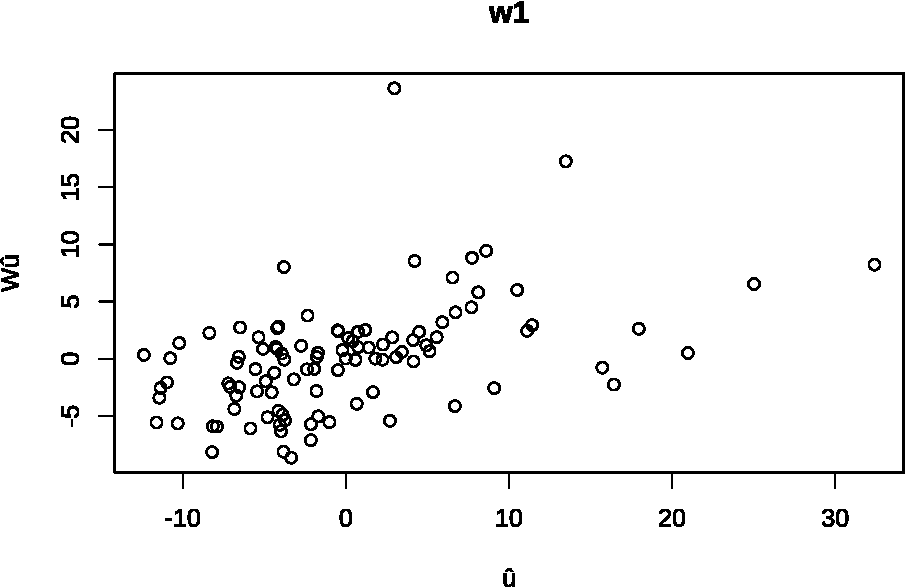
\includegraphics{assignment2_files/figure-latex/unnamed-chunk-14-1.pdf}

\begin{Shaded}
\begin{Highlighting}[]
\FunctionTok{plot}\NormalTok{(residuals, lagged\_residuals\_w2, }\AttributeTok{main =} \StringTok{"w2"}\NormalTok{, }\AttributeTok{xlab =} \StringTok{"û"}\NormalTok{, }\AttributeTok{ylab =} \StringTok{"Wû"}\NormalTok{)}
\end{Highlighting}
\end{Shaded}

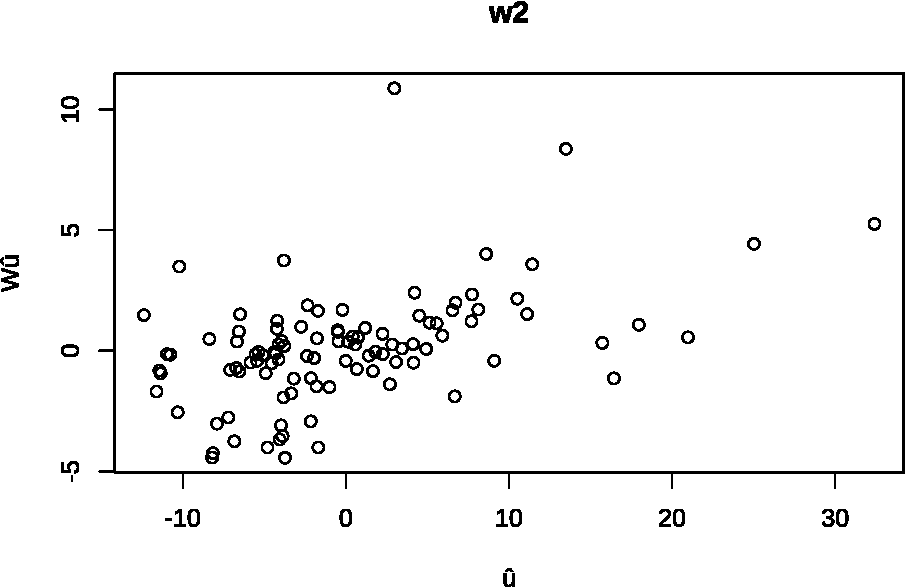
\includegraphics{assignment2_files/figure-latex/unnamed-chunk-14-2.pdf}

\begin{Shaded}
\begin{Highlighting}[]
\FunctionTok{plot}\NormalTok{(residuals, lagged\_residuals\_w3, }\AttributeTok{main =} \StringTok{"w3"}\NormalTok{, }\AttributeTok{xlab =} \StringTok{"û"}\NormalTok{, }\AttributeTok{ylab =} \StringTok{"Wû"}\NormalTok{)}
\end{Highlighting}
\end{Shaded}

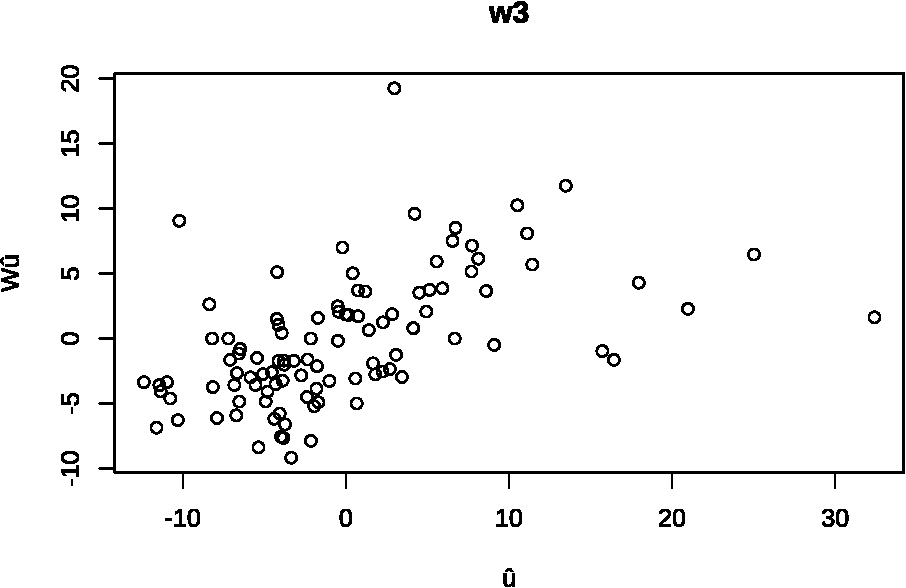
\includegraphics{assignment2_files/figure-latex/unnamed-chunk-14-3.pdf}

For all three weight matrices, we observe a slight positive relationship
between residuals and their spatially lagged counterparts, specially
when using \(W_3\), implying certain spatial autocorrelation between
residuals.

To statistically check for spatial autocorrelation, we can compute once
again Global Moran's I using each weight matrix, this time analyzing the
residuals instead of productivity growth.

\begin{Shaded}
\begin{Highlighting}[]
\NormalTok{iw1 }\OtherTok{\textless{}{-}} \FunctionTok{moran.test}\NormalTok{(residuals, w1listw)}
\NormalTok{iw1 }\OtherTok{\textless{}{-}}\NormalTok{ iw1}\SpecialCharTok{$}\NormalTok{estimate[}\StringTok{"Moran I statistic"}\NormalTok{]}

\NormalTok{iw2 }\OtherTok{\textless{}{-}} \FunctionTok{moran.test}\NormalTok{(residuals, w2listw)}
\NormalTok{iw2 }\OtherTok{\textless{}{-}}\NormalTok{ iw2}\SpecialCharTok{$}\NormalTok{estimate[}\StringTok{"Moran I statistic"}\NormalTok{]}

\NormalTok{iw3 }\OtherTok{\textless{}{-}} \FunctionTok{moran.test}\NormalTok{(residuals, w3listw)}
\NormalTok{iw3 }\OtherTok{\textless{}{-}}\NormalTok{ iw3}\SpecialCharTok{$}\NormalTok{estimate[}\StringTok{"Moran I statistic"}\NormalTok{]}

\NormalTok{I\_score\_comparison2 }\OtherTok{\textless{}{-}} \FunctionTok{c}\NormalTok{(iw1, iw2, iw3)}
\FunctionTok{names}\NormalTok{(I\_score\_comparison2) }\OtherTok{\textless{}{-}} \FunctionTok{c}\NormalTok{(}\StringTok{"w1"}\NormalTok{, }\StringTok{"w2"}\NormalTok{, }\StringTok{"w3"}\NormalTok{)}
\FunctionTok{print}\NormalTok{(I\_score\_comparison2)}
\end{Highlighting}
\end{Shaded}

\begin{verbatim}
##        w1        w2        w3 
## 0.2930808 0.1380220 0.3225208
\end{verbatim}

The statistics related to \(W_1\) and \(W_3\) imply a moderate level of
clustering of errors, whereas if we use \(W_2\) to check for spatial
autocorrelation, we would obtain a value indicating less clustering. The
presence of spatial dependence across errors implies that the assumption
of independent errors is violated. If we were to run an OLS regression,
our estimates would be biased and inconsistent.If we suspect that the
errors are spatially autocorrelated, we can use the spatial error model
(SEM), using a weight matrix to account for the autocorrelation.

On the other hand, if there is spatial dependence between the
observations of interest (in our case productivity growth rate), the
estimates obtained from a regression will not accurately capture the
true effect of the independent variable(s), since effects related to
spatial characteristics will be mistakenly attributed to the parameter.
In that case, we could estimate a spatial autoregressive model (SAR), in
which the neighbors' characteristics are also considered when estimating
the parameters.

\newpage

\section{Task B}\label{task-b}

\subsection{Nice Maps}\label{nice-maps}

We create four maps:

\begin{center}\includegraphics[width=0.7\linewidth]{assignment2_files/figure-latex/unnamed-chunk-16-1} \end{center}

\begin{center}\includegraphics[width=0.7\linewidth]{assignment2_files/figure-latex/unnamed-chunk-16-2} \end{center}

\begin{center}\includegraphics[width=0.7\linewidth]{assignment2_files/figure-latex/unnamed-chunk-16-3} \end{center}

\begin{center}\includegraphics[width=0.7\linewidth]{assignment2_files/figure-latex/unnamed-chunk-16-4} \end{center}

\subsection{Replication of Table 2}\label{replication-of-table-2}

Below are code and results of our replication of Table 2 from
\textcite{valencia2019}. Since the original author used Stata's robust
standard errors, a notorious problem for replication in R, we
specifically report Stata-style standard errors in the table below using
the \texttt{starprep} function from the \texttt{estimatr} package. Using
these standard errors, we can reproduce both coefficients and standard
errors exactly.

\begin{Shaded}
\begin{Highlighting}[]
\CommentTok{\# Replicate Results {-}{-}{-}{-}{-}{-}{-}{-}{-}{-}{-}{-}{-}{-}{-}{-}{-}{-}{-}{-}{-}{-}{-}{-}{-}{-}{-}{-}{-}{-}{-}{-}{-}{-}{-}{-}{-}{-}{-}{-}{-}{-}{-}{-}{-}{-}{-}{-}{-}{-}{-}{-}{-}{-}{-}}
\NormalTok{col1 }\OtherTok{\textless{}{-}} \FunctionTok{lm}\NormalTok{(illiteracy }\SpecialCharTok{\textasciitilde{}}\NormalTok{ distmiss }\SpecialCharTok{+}\NormalTok{ lati }\SpecialCharTok{+}\NormalTok{ longi }\SpecialCharTok{+}\NormalTok{ corr }\SpecialCharTok{+}\NormalTok{ ita }\SpecialCharTok{+}\NormalTok{ mis }\SpecialCharTok{+}\NormalTok{ mis1, }\AttributeTok{data =}\NormalTok{ litr)}
\NormalTok{col2 }\OtherTok{\textless{}{-}} \FunctionTok{lm}\NormalTok{(illiteracy }\SpecialCharTok{\textasciitilde{}}\NormalTok{ distmiss }\SpecialCharTok{+}\NormalTok{ lati }\SpecialCharTok{+}\NormalTok{ longi }\SpecialCharTok{+}\NormalTok{ area }\SpecialCharTok{+}\NormalTok{ tempe }\SpecialCharTok{+}\NormalTok{ alti }\SpecialCharTok{+}\NormalTok{ preci }\SpecialCharTok{+}\NormalTok{ rugg }\SpecialCharTok{+}
\NormalTok{    river }\SpecialCharTok{+}\NormalTok{ coast }\SpecialCharTok{+}\NormalTok{ corr }\SpecialCharTok{+}\NormalTok{ ita }\SpecialCharTok{+}\NormalTok{ mis }\SpecialCharTok{+}\NormalTok{ mis1, }\AttributeTok{data =}\NormalTok{ litr)}

\NormalTok{litr\_bra }\OtherTok{\textless{}{-}} \FunctionTok{subset}\NormalTok{(litr, country }\SpecialCharTok{==} \StringTok{"BRA"}\NormalTok{)}
\NormalTok{col3 }\OtherTok{\textless{}{-}} \FunctionTok{lm}\NormalTok{(illiteracy }\SpecialCharTok{\textasciitilde{}}\NormalTok{ distmiss }\SpecialCharTok{+}\NormalTok{ lati }\SpecialCharTok{+}\NormalTok{ longi }\SpecialCharTok{+} \FunctionTok{as.factor}\NormalTok{(mesorregi), }\AttributeTok{data =}\NormalTok{ litr\_bra)}
\NormalTok{col4 }\OtherTok{\textless{}{-}} \FunctionTok{lm}\NormalTok{(illiteracy }\SpecialCharTok{\textasciitilde{}}\NormalTok{ distmiss }\SpecialCharTok{+}\NormalTok{ lati }\SpecialCharTok{+}\NormalTok{ longi }\SpecialCharTok{+}\NormalTok{ area }\SpecialCharTok{+}\NormalTok{ tempe }\SpecialCharTok{+}\NormalTok{ alti }\SpecialCharTok{+}\NormalTok{ preci }\SpecialCharTok{+}\NormalTok{ rugg }\SpecialCharTok{+}
\NormalTok{    river }\SpecialCharTok{+}\NormalTok{ coast }\SpecialCharTok{+} \FunctionTok{as.factor}\NormalTok{(mesorregi), }\AttributeTok{data =}\NormalTok{ litr\_bra)}

\NormalTok{litr\_arg }\OtherTok{\textless{}{-}} \FunctionTok{subset}\NormalTok{(litr, country }\SpecialCharTok{==} \StringTok{"Argentina"}\NormalTok{)}
\NormalTok{col5 }\OtherTok{\textless{}{-}} \FunctionTok{lm}\NormalTok{(illiteracy }\SpecialCharTok{\textasciitilde{}}\NormalTok{ distmiss }\SpecialCharTok{+}\NormalTok{ lati }\SpecialCharTok{+}\NormalTok{ longi }\SpecialCharTok{+}\NormalTok{ corr, }\AttributeTok{data =}\NormalTok{ litr\_arg)}
\NormalTok{col6 }\OtherTok{\textless{}{-}} \FunctionTok{lm}\NormalTok{(illiteracy }\SpecialCharTok{\textasciitilde{}}\NormalTok{ distmiss }\SpecialCharTok{+}\NormalTok{ lati }\SpecialCharTok{+}\NormalTok{ longi }\SpecialCharTok{+}\NormalTok{ area }\SpecialCharTok{+}\NormalTok{ tempe }\SpecialCharTok{+}\NormalTok{ alti }\SpecialCharTok{+}\NormalTok{ preci }\SpecialCharTok{+}\NormalTok{ rugg }\SpecialCharTok{+}
\NormalTok{    river }\SpecialCharTok{+}\NormalTok{ coast }\SpecialCharTok{+}\NormalTok{ corr, }\AttributeTok{data =}\NormalTok{ litr\_arg)}

\NormalTok{litr\_pry }\OtherTok{\textless{}{-}} \FunctionTok{subset}\NormalTok{(litr, country }\SpecialCharTok{==} \StringTok{"Paraguay"}\NormalTok{)}
\NormalTok{col7 }\OtherTok{\textless{}{-}} \FunctionTok{lm}\NormalTok{(illiteracy }\SpecialCharTok{\textasciitilde{}}\NormalTok{ distmiss }\SpecialCharTok{+}\NormalTok{ ita, }\AttributeTok{data =}\NormalTok{ litr\_pry)}
\NormalTok{col8 }\OtherTok{\textless{}{-}} \FunctionTok{lm}\NormalTok{(illiteracy }\SpecialCharTok{\textasciitilde{}}\NormalTok{ distmiss }\SpecialCharTok{+}\NormalTok{ area }\SpecialCharTok{+}\NormalTok{ tempe }\SpecialCharTok{+}\NormalTok{ alti }\SpecialCharTok{+}\NormalTok{ preci }\SpecialCharTok{+}\NormalTok{ rugg }\SpecialCharTok{+}\NormalTok{ river }\SpecialCharTok{+}\NormalTok{ coast }\SpecialCharTok{+}
\NormalTok{    ita, }\AttributeTok{data =}\NormalTok{ litr\_pry)}
\end{Highlighting}
\end{Shaded}

\begin{center}\scalebox{.9}{
\begin{tabular}{@{\extracolsep{3pt}}lcccc} 
\\[-1.8ex]\hline 
\hline \\[-1.8ex] 
 & \multicolumn{4}{c}{\textit{Dependent variable:}} \\ 
\cline{2-5} 
\\[-1.8ex] & \multicolumn{4}{c}{illiteracy} \\ 
\\[-1.8ex] & (1) & (2) & (3) & (4)\\ 
\hline \\[-1.8ex] 
 distmiss & 0.011$^{***}$ & 0.011$^{**}$ & 0.016$^{*}$ & 0.030$^{***}$ \\ 
  & (0.004) & (0.005) & (0.009) & (0.010) \\ 
  lati & 0.556$^{**}$ & 0.070 & 0.408 & 4.575$^{**}$ \\ 
  & (0.238) & (0.781) & (0.553) & (1.807) \\ 
  longi & $-$1.108$^{***}$ & $-$1.007$^{*}$ & $-$1.022 & $-$5.694$^{***}$ \\ 
  & (0.257) & (0.556) & (0.689) & (1.811) \\ 
  area &  & 0.0001 &  & $-$0.0002 \\ 
  &  & (0.0002) &  & (0.0004) \\ 
  tempe &  & 0.059 &  & $-$0.062 \\ 
  &  & (0.077) &  & (0.124) \\ 
  alti &  & 0.006 &  & 0.001 \\ 
  &  & (0.004) &  & (0.005) \\ 
  preci &  & $-$0.003 &  & 0.001 \\ 
  &  & (0.002) &  & (0.003) \\ 
  rugg &  & $-$0.00000 &  & $-$0.00000 \\ 
  &  & (0.00000) &  & (0.00000) \\ 
  river &  & 1.470$^{**}$ &  & 1.723$^{*}$ \\ 
  &  & (0.712) &  & (0.893) \\ 
  coast &  & 0.209 &  & $-$4.976$^{**}$ \\ 
  &  & (0.894) &  & (2.147) \\ 
  corr & $-$5.341$^{***}$ & $-$6.032$^{***}$ &  &  \\ 
  & (1.286) & (1.583) &  &  \\ 
  ita & $-$3.187$^{***}$ & $-$2.409$^{***}$ &  &  \\ 
  & (0.728) & (0.833) &  &  \\ 
  mis & $-$4.324$^{***}$ & $-$4.734$^{***}$ &  &  \\ 
  & (1.122) & (1.488) &  &  \\ 
  mis1 & $-$3.279$^{***}$ & $-$2.299$^{**}$ &  &  \\ 
  & (0.860) & (0.974) &  &  \\ 
  as.factor(mesorregi)4302 &  &  & $-$2.720$^{***}$ & $-$2.543$^{**}$ \\ 
  &  &  & (0.863) & (1.037) \\ 
  as.factor(mesorregi)4303 &  &  & $-$0.483 & $-$0.383 \\ 
  &  &  & (1.133) & (1.228) \\ 
  as.factor(mesorregi)4304 &  &  & $-$0.771 & 0.196 \\ 
  &  &  & (1.150) & (1.403) \\ 
  as.factor(mesorregi)4305 &  &  & $-$3.023$^{**}$ & $-$1.290 \\ 
  &  &  & (1.312) & (1.541) \\ 
  as.factor(mesorregi)4306 &  &  & $-$1.724 & $-$3.421 \\ 
  &  &  & (2.015) & (2.184) \\ 
  as.factor(mesorregi)4307 &  &  & $-$0.437 & 0.327 \\ 
  &  &  & (2.553) & (2.634) \\ 
  Constant & $-$35.328$^{***}$ & $-$53.741$^{*}$ & $-$35.274 & $-$143.869$^{**}$ \\ 
  & (11.797) & (32.497) & (38.125) & (66.532) \\ 
 \hline \\[-1.8ex] 
Observations & 549 & 548 & 467 & 467 \\ 
R$^{2}$ & 0.042 & 0.073 & 0.094 & 0.135 \\ 
Adjusted R$^{2}$ & 0.029 & 0.049 & 0.076 & 0.104 \\ 
Residual Std. Error & 3.948 (df = 541) & 3.912 (df = 533) & 4.040 (df = 457) & 3.978 (df = 450) \\ 
\hline 
\hline \\[-1.8ex] 
\textit{Note:}  & \multicolumn{4}{r}{$^{*}$p$<$0.1; $^{**}$p$<$0.05; $^{***}$p$<$0.01} \\ 
\end{tabular} 
}\end{center}

\begin{center}\scalebox{.9}{
\begin{tabular}{@{\extracolsep{3pt}}lcccc} 
\\[-1.8ex]\hline 
\hline \\[-1.8ex] 
 & \multicolumn{4}{c}{\textit{Dependent variable:}} \\ 
\cline{2-5} 
\\[-1.8ex] & \multicolumn{4}{c}{illiteracy} \\ 
 & (5) & (6) & (7) & (8) \\ 
\hline \\[-1.8ex] 
 distmiss & 0.016$^{**}$ & 0.067$^{***}$ & 0.005 & 0.014 \\ 
  & (0.007) & (0.022) & (0.012) & (0.027) \\ 
  lati & 0.084 & $-$9.338$^{**}$ &  &  \\ 
  & (0.758) & (3.831) &  &  \\ 
  longi & 1.095 & 7.186$^{***}$ &  &  \\ 
  & (0.803) & (2.676) &  &  \\ 
  area &  & $-$0.0001 &  & 0.0004 \\ 
  &  & (0.0003) &  & (0.001) \\ 
  tempe &  & 0.968$^{***}$ &  & 0.360 \\ 
  &  & (0.237) &  & (0.220) \\ 
  alti &  & 0.065$^{***}$ &  & 0.016 \\ 
  &  & (0.011) &  & (0.014) \\ 
  preci &  & $-$0.017$^{**}$ &  & 0.0001 \\ 
  &  & (0.008) &  & (0.005) \\ 
  rugg &  & $-$0.00005$^{***}$ &  & 0.0001 \\ 
  &  & (0.00002) &  & (0.00005) \\ 
  river &  & 9.795$^{***}$ &  & 0.983 \\ 
  &  & (2.173) &  & (5.492) \\ 
  coast &  & 1.889 &  & 0.826 \\ 
  &  & (3.522) &  & (4.557) \\ 
  corr & 3.771$^{**}$ & $-$3.043 &  &  \\ 
  & (1.850) & (3.644) &  &  \\ 
  ita &  &  & $-$0.231 & 0.829 \\ 
  &  &  & (0.832) & (2.316) \\ 
  Constant & 69.263$^{*}$ & $-$41.058 & 8.673$^{***}$ & $-$80.723$^{*}$ \\ 
  & (36.792) & (54.628) & (0.694) & (43.888) \\ 
 \hline \\[-1.8ex] 
Observations & 42 & 42 & 40 & 39 \\ 
R$^{2}$ & 0.165 & 0.669 & 0.004 & 0.251 \\ 
Adjusted R$^{2}$ & 0.075 & 0.547 & $-$0.050 & 0.019 \\ 
Residual Std. Error & 2.924 (df = 37) & 2.045 (df = 30) & 2.150 (df = 37) & 2.101 (df = 29) \\ 
\hline 
\hline \\[-1.8ex] 
\textit{Note:}  & \multicolumn{4}{r}{$^{*}$p$<$0.1; $^{**}$p$<$0.05; $^{***}$p$<$0.01} \\ 
\end{tabular} 
}\end{center}

Next, we try to reproduce the Conley standard errors. We try two
different approaches, first using the \texttt{conleyreg} package and
then using the \texttt{fixest} package. \textcite{valencia2019}
specifies a cutoff distance of 0.1 degrees. Both packages we use only
allow us to specify the cutoff distance in kilometers, so for the sake
of simplicity, we use the distance that 0.1 degrees equal at the
equator, which is 6 nautical miles, or approximately 11.112 kilometers.
We first print the results from the \texttt{conleyreg} package and then
from the \texttt{fixest} package.

\begin{Shaded}
\begin{Highlighting}[]
\NormalTok{lit1 }\OtherTok{\textless{}{-}}\NormalTok{ litr }\SpecialCharTok{\%\textgreater{}\%}
    \FunctionTok{drop\_na}\NormalTok{(lati, longi) }\SpecialCharTok{\%\textgreater{}\%}
    \FunctionTok{mutate}\NormalTok{(}\AttributeTok{lat =}\NormalTok{ lati, }\AttributeTok{lon =}\NormalTok{ longi)}

\NormalTok{col1c }\OtherTok{\textless{}{-}} \FunctionTok{conleyreg}\NormalTok{(illiteracy }\SpecialCharTok{\textasciitilde{}}\NormalTok{ distmiss }\SpecialCharTok{+}\NormalTok{ lati }\SpecialCharTok{+}\NormalTok{ longi }\SpecialCharTok{+}\NormalTok{ corr }\SpecialCharTok{+}\NormalTok{ ita }\SpecialCharTok{+}\NormalTok{ mis }\SpecialCharTok{+}\NormalTok{ mis1,}
    \AttributeTok{data =}\NormalTok{ lit1, }\AttributeTok{dist\_cutoff =} \FloatTok{11.112}\NormalTok{, }\AttributeTok{lat =} \StringTok{"lat"}\NormalTok{, }\AttributeTok{lon =} \StringTok{"lon"}\NormalTok{)}
\NormalTok{col2c }\OtherTok{\textless{}{-}} \FunctionTok{conleyreg}\NormalTok{(illiteracy }\SpecialCharTok{\textasciitilde{}}\NormalTok{ distmiss }\SpecialCharTok{+}\NormalTok{ lati }\SpecialCharTok{+}\NormalTok{ longi }\SpecialCharTok{+}\NormalTok{ area }\SpecialCharTok{+}\NormalTok{ tempe }\SpecialCharTok{+}\NormalTok{ alti }\SpecialCharTok{+}\NormalTok{ preci }\SpecialCharTok{+}
\NormalTok{    rugg }\SpecialCharTok{+}\NormalTok{ river }\SpecialCharTok{+}\NormalTok{ coast }\SpecialCharTok{+}\NormalTok{ corr }\SpecialCharTok{+}\NormalTok{ ita }\SpecialCharTok{+}\NormalTok{ mis }\SpecialCharTok{+}\NormalTok{ mis1, }\AttributeTok{data =}\NormalTok{ lit1, }\AttributeTok{dist\_cutoff =} \FloatTok{11.112}\NormalTok{,}
    \AttributeTok{lat =} \StringTok{"lat"}\NormalTok{, }\AttributeTok{lon =} \StringTok{"lon"}\NormalTok{)}

\NormalTok{lit1\_bra }\OtherTok{\textless{}{-}} \FunctionTok{subset}\NormalTok{(lit1, country }\SpecialCharTok{==} \StringTok{"BRA"}\NormalTok{)}
\NormalTok{col3c }\OtherTok{\textless{}{-}} \FunctionTok{conleyreg}\NormalTok{(illiteracy }\SpecialCharTok{\textasciitilde{}}\NormalTok{ distmiss }\SpecialCharTok{+}\NormalTok{ lati }\SpecialCharTok{+}\NormalTok{ longi }\SpecialCharTok{+} \FunctionTok{as.factor}\NormalTok{(mesorregi), }\AttributeTok{data =}\NormalTok{ lit1\_bra,}
    \AttributeTok{dist\_cutoff =} \FloatTok{11.112}\NormalTok{, }\AttributeTok{lat =} \StringTok{"lat"}\NormalTok{, }\AttributeTok{lon =} \StringTok{"lon"}\NormalTok{)}
\NormalTok{col4c }\OtherTok{\textless{}{-}} \FunctionTok{conleyreg}\NormalTok{(illiteracy }\SpecialCharTok{\textasciitilde{}}\NormalTok{ distmiss }\SpecialCharTok{+}\NormalTok{ lati }\SpecialCharTok{+}\NormalTok{ longi }\SpecialCharTok{+}\NormalTok{ area }\SpecialCharTok{+}\NormalTok{ tempe }\SpecialCharTok{+}\NormalTok{ alti }\SpecialCharTok{+}\NormalTok{ preci }\SpecialCharTok{+}
\NormalTok{    rugg }\SpecialCharTok{+}\NormalTok{ river }\SpecialCharTok{+}\NormalTok{ coast }\SpecialCharTok{+} \FunctionTok{as.factor}\NormalTok{(mesorregi), }\AttributeTok{data =}\NormalTok{ lit1\_bra, }\AttributeTok{dist\_cutoff =} \FloatTok{11.112}\NormalTok{,}
    \AttributeTok{lat =} \StringTok{"lat"}\NormalTok{, }\AttributeTok{lon =} \StringTok{"lon"}\NormalTok{)}

\NormalTok{lit1\_arg }\OtherTok{\textless{}{-}} \FunctionTok{subset}\NormalTok{(lit1, country }\SpecialCharTok{==} \StringTok{"Argentina"}\NormalTok{)}
\NormalTok{col5c }\OtherTok{\textless{}{-}} \FunctionTok{conleyreg}\NormalTok{(illiteracy }\SpecialCharTok{\textasciitilde{}}\NormalTok{ distmiss }\SpecialCharTok{+}\NormalTok{ lati }\SpecialCharTok{+}\NormalTok{ longi }\SpecialCharTok{+}\NormalTok{ corr, }\AttributeTok{data =}\NormalTok{ lit1\_arg,}
    \AttributeTok{dist\_cutoff =} \FloatTok{11.112}\NormalTok{, }\AttributeTok{lat =} \StringTok{"lat"}\NormalTok{, }\AttributeTok{lon =} \StringTok{"lon"}\NormalTok{)}
\NormalTok{col6c }\OtherTok{\textless{}{-}} \FunctionTok{conleyreg}\NormalTok{(illiteracy }\SpecialCharTok{\textasciitilde{}}\NormalTok{ distmiss }\SpecialCharTok{+}\NormalTok{ lati }\SpecialCharTok{+}\NormalTok{ longi }\SpecialCharTok{+}\NormalTok{ area }\SpecialCharTok{+}\NormalTok{ tempe }\SpecialCharTok{+}\NormalTok{ alti }\SpecialCharTok{+}\NormalTok{ preci }\SpecialCharTok{+}
\NormalTok{    rugg }\SpecialCharTok{+}\NormalTok{ river }\SpecialCharTok{+}\NormalTok{ coast }\SpecialCharTok{+}\NormalTok{ corr, }\AttributeTok{data =}\NormalTok{ lit1\_arg, }\AttributeTok{dist\_cutoff =} \FloatTok{11.112}\NormalTok{, }\AttributeTok{lat =} \StringTok{"lat"}\NormalTok{,}
    \AttributeTok{lon =} \StringTok{"lon"}\NormalTok{)}

\NormalTok{lit1\_pry }\OtherTok{\textless{}{-}} \FunctionTok{subset}\NormalTok{(lit1, country }\SpecialCharTok{==} \StringTok{"Paraguay"}\NormalTok{)}
\NormalTok{col7c }\OtherTok{\textless{}{-}} \FunctionTok{conleyreg}\NormalTok{(illiteracy }\SpecialCharTok{\textasciitilde{}}\NormalTok{ distmiss }\SpecialCharTok{+}\NormalTok{ ita, }\AttributeTok{data =}\NormalTok{ lit1\_pry, }\AttributeTok{dist\_cutoff =} \FloatTok{11.112}\NormalTok{,}
    \AttributeTok{lat =} \StringTok{"lat"}\NormalTok{, }\AttributeTok{lon =} \StringTok{"lon"}\NormalTok{)}
\NormalTok{col8c }\OtherTok{\textless{}{-}} \FunctionTok{conleyreg}\NormalTok{(illiteracy }\SpecialCharTok{\textasciitilde{}}\NormalTok{ distmiss }\SpecialCharTok{+}\NormalTok{ area }\SpecialCharTok{+}\NormalTok{ tempe }\SpecialCharTok{+}\NormalTok{ alti }\SpecialCharTok{+}\NormalTok{ preci }\SpecialCharTok{+}\NormalTok{ rugg }\SpecialCharTok{+}\NormalTok{ river }\SpecialCharTok{+}
\NormalTok{    coast }\SpecialCharTok{+}\NormalTok{ ita, }\AttributeTok{data =}\NormalTok{ lit1\_pry, }\AttributeTok{dist\_cutoff =} \FloatTok{11.112}\NormalTok{, }\AttributeTok{lat =} \StringTok{"lat"}\NormalTok{, }\AttributeTok{lon =} \StringTok{"lon"}\NormalTok{)}
\end{Highlighting}
\end{Shaded}

\begin{center}\scalebox{.9}{
\begin{tabular}{@{\extracolsep{3pt}}lcccc} 
\\[-1.8ex]\hline 
\hline \\[-1.8ex] 
 & \multicolumn{4}{c}{\textit{Dependent variable:}} \\ 
\cline{2-5} 
\\[-1.8ex] & \multicolumn{4}{c}{ } \\ 
\\[-1.8ex] & (1) & (2) & (3) & (4)\\ 
\hline \\[-1.8ex] 
 distmiss & 0.011$^{***}$ & 0.011$^{**}$ & 0.016$^{*}$ & 0.030$^{***}$ \\ 
  & (0.004) & (0.005) & (0.009) & (0.010) \\ 
  lati & 0.556$^{**}$ & 0.070 & 0.408 & 4.575$^{**}$ \\ 
  & (0.247) & (0.773) & (0.570) & (1.792) \\ 
  longi & $-$1.108$^{***}$ & $-$1.007$^{*}$ & $-$1.022 & $-$5.694$^{***}$ \\ 
  & (0.266) & (0.549) & (0.696) & (1.780) \\ 
  area &  & 0.0001 &  & $-$0.0002 \\ 
  &  & (0.0002) &  & (0.0003) \\ 
  tempe &  & 0.059 &  & $-$0.062 \\ 
  &  & (0.080) &  & (0.130) \\ 
  alti &  & 0.006 &  & 0.001 \\ 
  &  & (0.004) &  & (0.006) \\ 
  preci &  & $-$0.003 &  & 0.001 \\ 
  &  & (0.002) &  & (0.003) \\ 
  rugg &  & $-$0.00000 &  & $-$0.00000 \\ 
  &  & (0.00000) &  & (0.00000) \\ 
  river &  & 1.470$^{**}$ &  & 1.723$^{*}$ \\ 
  &  & (0.731) &  & (0.904) \\ 
  coast &  & 0.209 &  & $-$4.976$^{**}$ \\ 
  &  & (0.885) &  & (2.125) \\ 
  corr & $-$5.341$^{***}$ & $-$6.032$^{***}$ &  &  \\ 
  & (1.325) & (1.612) &  &  \\ 
  ita & $-$3.187$^{***}$ & $-$2.409$^{***}$ &  &  \\ 
  & (0.758) & (0.848) &  &  \\ 
  mis & $-$4.324$^{***}$ & $-$4.734$^{***}$ &  &  \\ 
  & (1.159) & (1.519) &  &  \\ 
  mis1 & $-$3.279$^{***}$ & $-$2.299$^{**}$ &  &  \\ 
  & (0.876) & (0.980) &  &  \\ 
  as.factor(mesorregi)4302 &  &  & $-$2.720$^{***}$ & $-$2.543$^{**}$ \\ 
  &  &  & (0.896) & (1.067) \\ 
  as.factor(mesorregi)4303 &  &  & $-$0.483 & $-$0.383 \\ 
  &  &  & (1.150) & (1.250) \\ 
  as.factor(mesorregi)4304 &  &  & $-$0.771 & 0.196 \\ 
  &  &  & (1.215) & (1.448) \\ 
  as.factor(mesorregi)4305 &  &  & $-$3.023$^{**}$ & $-$1.290 \\ 
  &  &  & (1.393) & (1.659) \\ 
  as.factor(mesorregi)4306 &  &  & $-$1.724 & $-$3.421 \\ 
  &  &  & (2.027) & (2.190) \\ 
  as.factor(mesorregi)4307 &  &  & $-$0.437 & 0.327 \\ 
  &  &  & (2.576) & (2.654) \\ 
  Constant & $-$35.328$^{***}$ & $-$53.741 & $-$35.274 & $-$143.869$^{**}$ \\ 
  & (12.074) & (33.356) & (38.313) & (66.608) \\ 
 \hline \\[-1.8ex] 
\hline 
\hline \\[-1.8ex] 
\textit{Note:}  & \multicolumn{4}{r}{$^{*}$p$<$0.1; $^{**}$p$<$0.05; $^{***}$p$<$0.01} \\ 
\end{tabular} 
}\end{center}

\begin{center}\scalebox{.9}{
\begin{tabular}{@{\extracolsep{3pt}}lcccc} 
\\[-1.8ex]\hline 
\hline \\[-1.8ex] 
 & \multicolumn{4}{c}{\textit{Dependent variable:}} \\ 
\cline{2-5} 
\\[-1.8ex] & \multicolumn{4}{c}{ } \\ 
 & (5) & (6) & (7) & (8) \\ 
\hline \\[-1.8ex] 
 distmiss & 0.016$^{**}$ & 0.067$^{***}$ & 0.005 & 0.014 \\ 
  & (0.007) & (0.019) & (0.011) & (0.023) \\ 
  lati & 0.084 & $-$9.338$^{***}$ &  &  \\ 
  & (0.711) & (3.238) &  &  \\ 
  longi & 1.095 & 7.186$^{***}$ &  &  \\ 
  & (0.754) & (2.262) &  &  \\ 
  area &  & $-$0.0001 &  & 0.0004 \\ 
  &  & (0.0002) &  & (0.001) \\ 
  tempe &  & 0.968$^{***}$ &  & 0.360$^{*}$ \\ 
  &  & (0.200) &  & (0.190) \\ 
  alti &  & 0.065$^{***}$ &  & 0.016 \\ 
  &  & (0.010) &  & (0.012) \\ 
  preci &  & $-$0.017$^{**}$ &  & 0.0001 \\ 
  &  & (0.007) &  & (0.004) \\ 
  rugg &  & $-$0.00005$^{***}$ &  & 0.0001 \\ 
  &  & (0.00002) &  & (0.00004) \\ 
  river &  & 9.795$^{***}$ &  & 0.983 \\ 
  &  & (1.837) &  & (4.738) \\ 
  coast &  & 1.889 &  & 0.826 \\ 
  &  & (2.976) &  & (3.941) \\ 
  corr & 3.771$^{**}$ & $-$3.043 &  &  \\ 
  & (1.736) & (3.080) &  &  \\ 
  ita &  &  & $-$0.231 & 0.829 \\ 
  &  &  & (0.794) & (1.998) \\ 
  Constant & 69.263$^{*}$ & $-$41.058 & 8.673$^{***}$ & $-$80.723$^{**}$ \\ 
  & (34.532) & (46.169) & (0.666) & (37.732) \\ 
 \hline \\[-1.8ex] 
\hline 
\hline \\[-1.8ex] 
\textit{Note:}  & \multicolumn{4}{r}{$^{*}$p$<$0.1; $^{**}$p$<$0.05; $^{***}$p$<$0.01} \\ 
\end{tabular} 
}\end{center}

\begin{Shaded}
\begin{Highlighting}[]
\NormalTok{col1cf }\OtherTok{\textless{}{-}} \FunctionTok{feols}\NormalTok{(illiteracy }\SpecialCharTok{\textasciitilde{}}\NormalTok{ distmiss }\SpecialCharTok{+}\NormalTok{ lati }\SpecialCharTok{+}\NormalTok{ longi }\SpecialCharTok{+}\NormalTok{ corr }\SpecialCharTok{+}\NormalTok{ ita }\SpecialCharTok{+}\NormalTok{ mis }\SpecialCharTok{+}\NormalTok{ mis1, }\AttributeTok{data =}\NormalTok{ litr,}
    \FunctionTok{vcov\_conley}\NormalTok{(}\AttributeTok{lat =} \StringTok{"lati"}\NormalTok{, }\AttributeTok{lon =} \StringTok{"longi"}\NormalTok{, }\AttributeTok{cutoff =} \FloatTok{11.112}\NormalTok{, }\AttributeTok{distance =} \StringTok{"spherical"}\NormalTok{))}
\NormalTok{col2cf }\OtherTok{\textless{}{-}} \FunctionTok{feols}\NormalTok{(illiteracy }\SpecialCharTok{\textasciitilde{}}\NormalTok{ distmiss }\SpecialCharTok{+}\NormalTok{ lati }\SpecialCharTok{+}\NormalTok{ longi }\SpecialCharTok{+}\NormalTok{ area }\SpecialCharTok{+}\NormalTok{ tempe }\SpecialCharTok{+}\NormalTok{ alti }\SpecialCharTok{+}\NormalTok{ preci }\SpecialCharTok{+}
\NormalTok{    rugg }\SpecialCharTok{+}\NormalTok{ river }\SpecialCharTok{+}\NormalTok{ coast }\SpecialCharTok{+}\NormalTok{ corr }\SpecialCharTok{+}\NormalTok{ ita }\SpecialCharTok{+}\NormalTok{ mis }\SpecialCharTok{+}\NormalTok{ mis1, }\AttributeTok{data =}\NormalTok{ litr, }\FunctionTok{vcov\_conley}\NormalTok{(}\AttributeTok{lat =} \StringTok{"lati"}\NormalTok{,}
    \AttributeTok{lon =} \StringTok{"longi"}\NormalTok{, }\AttributeTok{cutoff =} \FloatTok{11.112}\NormalTok{, }\AttributeTok{distance =} \StringTok{"spherical"}\NormalTok{))}

\NormalTok{col3cf }\OtherTok{\textless{}{-}} \FunctionTok{feols}\NormalTok{(illiteracy }\SpecialCharTok{\textasciitilde{}}\NormalTok{ distmiss }\SpecialCharTok{+}\NormalTok{ lati }\SpecialCharTok{+}\NormalTok{ longi }\SpecialCharTok{+} \FunctionTok{as.factor}\NormalTok{(mesorregi), }\AttributeTok{data =}\NormalTok{ litr\_bra,}
    \FunctionTok{vcov\_conley}\NormalTok{(}\AttributeTok{lat =} \StringTok{"lati"}\NormalTok{, }\AttributeTok{lon =} \StringTok{"longi"}\NormalTok{, }\AttributeTok{cutoff =} \FloatTok{11.112}\NormalTok{, }\AttributeTok{distance =} \StringTok{"spherical"}\NormalTok{))}
\NormalTok{col4cf }\OtherTok{\textless{}{-}} \FunctionTok{feols}\NormalTok{(illiteracy }\SpecialCharTok{\textasciitilde{}}\NormalTok{ distmiss }\SpecialCharTok{+}\NormalTok{ lati }\SpecialCharTok{+}\NormalTok{ longi }\SpecialCharTok{+}\NormalTok{ area }\SpecialCharTok{+}\NormalTok{ tempe }\SpecialCharTok{+}\NormalTok{ alti }\SpecialCharTok{+}\NormalTok{ preci }\SpecialCharTok{+}
\NormalTok{    rugg }\SpecialCharTok{+}\NormalTok{ river }\SpecialCharTok{+}\NormalTok{ coast }\SpecialCharTok{+} \FunctionTok{as.factor}\NormalTok{(mesorregi), }\AttributeTok{data =}\NormalTok{ litr\_bra, }\FunctionTok{vcov\_conley}\NormalTok{(}\AttributeTok{lat =} \StringTok{"lati"}\NormalTok{,}
    \AttributeTok{lon =} \StringTok{"longi"}\NormalTok{, }\AttributeTok{cutoff =} \FloatTok{11.112}\NormalTok{, }\AttributeTok{distance =} \StringTok{"spherical"}\NormalTok{))}

\NormalTok{col5cf }\OtherTok{\textless{}{-}} \FunctionTok{feols}\NormalTok{(illiteracy }\SpecialCharTok{\textasciitilde{}}\NormalTok{ distmiss }\SpecialCharTok{+}\NormalTok{ lati }\SpecialCharTok{+}\NormalTok{ longi }\SpecialCharTok{+}\NormalTok{ corr, }\AttributeTok{data =}\NormalTok{ litr\_arg, }\FunctionTok{vcov\_conley}\NormalTok{(}\AttributeTok{lat =} \StringTok{"lati"}\NormalTok{,}
    \AttributeTok{lon =} \StringTok{"longi"}\NormalTok{, }\AttributeTok{cutoff =} \FloatTok{11.112}\NormalTok{, }\AttributeTok{distance =} \StringTok{"spherical"}\NormalTok{))}
\NormalTok{col6cf }\OtherTok{\textless{}{-}} \FunctionTok{feols}\NormalTok{(illiteracy }\SpecialCharTok{\textasciitilde{}}\NormalTok{ distmiss }\SpecialCharTok{+}\NormalTok{ lati }\SpecialCharTok{+}\NormalTok{ longi }\SpecialCharTok{+}\NormalTok{ area }\SpecialCharTok{+}\NormalTok{ tempe }\SpecialCharTok{+}\NormalTok{ alti }\SpecialCharTok{+}\NormalTok{ preci }\SpecialCharTok{+}
\NormalTok{    rugg }\SpecialCharTok{+}\NormalTok{ river }\SpecialCharTok{+}\NormalTok{ coast }\SpecialCharTok{+}\NormalTok{ corr, }\AttributeTok{data =}\NormalTok{ litr\_arg, }\FunctionTok{vcov\_conley}\NormalTok{(}\AttributeTok{lat =} \StringTok{"lati"}\NormalTok{, }\AttributeTok{lon =} \StringTok{"longi"}\NormalTok{,}
    \AttributeTok{cutoff =} \FloatTok{11.112}\NormalTok{, }\AttributeTok{distance =} \StringTok{"spherical"}\NormalTok{))}

\NormalTok{col7cf }\OtherTok{\textless{}{-}} \FunctionTok{feols}\NormalTok{(illiteracy }\SpecialCharTok{\textasciitilde{}}\NormalTok{ distmiss }\SpecialCharTok{+}\NormalTok{ ita, }\AttributeTok{data =}\NormalTok{ litr\_pry, }\FunctionTok{vcov\_conley}\NormalTok{(}\AttributeTok{lat =} \StringTok{"lati"}\NormalTok{,}
    \AttributeTok{lon =} \StringTok{"longi"}\NormalTok{, }\AttributeTok{cutoff =} \FloatTok{11.112}\NormalTok{, }\AttributeTok{distance =} \StringTok{"spherical"}\NormalTok{))}
\NormalTok{col8cf }\OtherTok{\textless{}{-}} \FunctionTok{feols}\NormalTok{(illiteracy }\SpecialCharTok{\textasciitilde{}}\NormalTok{ distmiss }\SpecialCharTok{+}\NormalTok{ area }\SpecialCharTok{+}\NormalTok{ tempe }\SpecialCharTok{+}\NormalTok{ alti }\SpecialCharTok{+}\NormalTok{ preci }\SpecialCharTok{+}\NormalTok{ rugg }\SpecialCharTok{+}\NormalTok{ river }\SpecialCharTok{+}
\NormalTok{    coast }\SpecialCharTok{+}\NormalTok{ ita, }\AttributeTok{data =}\NormalTok{ litr\_pry, }\FunctionTok{vcov\_conley}\NormalTok{(}\AttributeTok{lat =} \StringTok{"lati"}\NormalTok{, }\AttributeTok{lon =} \StringTok{"longi"}\NormalTok{, }\AttributeTok{cutoff =} \FloatTok{11.112}\NormalTok{,}
    \AttributeTok{distance =} \StringTok{"spherical"}\NormalTok{))}
\end{Highlighting}
\end{Shaded}

\scalebox{.8}{\begingroup
\centering
\begin{tabular}{lcccccccc}
   \tabularnewline \midrule \midrule
   Dependent Variable: & \multicolumn{8}{c}{illiteracy}\\
   Model:                   & (1)            & (2)                    & (3)           & (4)                     & (5)           & (6)                          & (7)           & (8)\\  
   \midrule
   \emph{Variables}\\
   Constant                 & -35.33$^{***}$ & -53.74                 & -35.27        & -143.9$^{*}$            & 69.26$^{*}$   & -41.06                       & 8.673$^{***}$ & -80.72$^{*}$\\   
                            & (12.96)        & (38.28)                & (40.26)       & (73.54)                 & (36.35)       & (53.97)                      & (0.6825)      & (43.22)\\   
   distmiss                 & 0.0105$^{***}$ & 0.0112$^{*}$           & 0.0164$^{*}$  & 0.0297$^{**}$           & 0.0157$^{**}$ & 0.0669$^{***}$               & 0.0045        & 0.0138\\   
                            & (0.0040)       & (0.0057)               & (0.0092)      & (0.0115)                & (0.0073)      & (0.0217)                     & (0.0112)      & (0.0261)\\   
   lati                     & 0.5561$^{*}$   & 0.0698                 & 0.4078        & 4.575$^{**}$            & 0.0837        & -9.338$^{**}$                &               &   \\   
                            & (0.2841)       & (0.7983)               & (0.6512)      & (1.898)                 & (0.7486)      & (3.785)                      &               &   \\   
   longi                    & -1.108$^{***}$ & -1.007$^{*}$           & -1.022        & -5.694$^{***}$          & 1.095         & 7.186$^{**}$                 &               &   \\   
                            & (0.2957)       & (0.5727)               & (0.7468)      & (1.857)                 & (0.7939)      & (2.644)                      &               &   \\   
   corr                     & -5.341$^{***}$ & -6.032$^{***}$         &               &                         & 3.771$^{**}$  & -3.043                       &               &   \\   
                            & (1.462)        & (1.776)                &               &                         & (1.828)       & (3.600)                      &               &   \\   
   ita                      & -3.187$^{***}$ & -2.409$^{**}$          &               &                         &               &                              & -0.2311       & 0.8290\\   
                            & (0.8686)       & (0.9485)               &               &                         &               &                              & (0.8123)      & (2.294)\\   
   mis                      & -4.324$^{***}$ & -4.734$^{***}$         &               &                         &               &                              &               &   \\   
                            & (1.289)        & (1.695)                &               &                         &               &                              &               &   \\   
   mis1                     & -3.279$^{***}$ & -2.299$^{**}$          &               &                         &               &                              &               &   \\   
                            & (0.9438)       & (1.042)                &               &                         &               &                              &               &   \\   
   area                     &                & 0.0001                 &               & -0.0002                 &               & $-8.9\times 10^{-5}$         &               & 0.0004\\   
                            &                & (0.0002)               &               & (0.0004)                &               & (0.0003)                     &               & (0.0007)\\   
   tempe                    &                & 0.0587                 &               & -0.0625                 &               & 0.9675$^{***}$               &               & 0.3598\\   
                            &                & (0.0937)               &               & (0.1558)                &               & (0.2343)                     &               & (0.2205)\\   
   alti                     &                & 0.0057                 &               & 0.0006                  &               & 0.0654$^{***}$               &               & 0.0160\\   
                            &                & (0.0042)               &               & (0.0067)                &               & (0.0112)                     &               & (0.0137)\\   
   preci                    &                & -0.0026                &               & 0.0010                  &               & -0.0171$^{**}$               &               & 0.0001\\   
                            &                & (0.0027)               &               & (0.0037)                &               & (0.0083)                     &               & (0.0051)\\   
   rugg                     &                & $-3.56\times 10^{-6}$  &               & $-3.09\times 10^{-6}$   &               & $-4.8\times 10^{-5}$$^{**}$  &               & $6.93\times 10^{-5}$\\    
                            &                & ($4.8\times 10^{-6}$)  &               & ($4.71\times 10^{-6}$)  &               & ($1.82\times 10^{-5}$)       &               & ($4.85\times 10^{-5}$)\\    
   river                    &                & 1.470$^{*}$            &               & 1.723$^{*}$             &               & 9.795$^{***}$                &               & 0.9834\\   
                            &                & (0.8202)               &               & (1.011)                 &               & (2.147)                      &               & (5.445)\\   
   coast                    &                & 0.2086                 &               & -4.976$^{**}$           &               & 1.889                        &               & 0.8264\\   
                            &                & (0.9177)               &               & (2.244)                 &               & (3.480)                      &               & (4.543)\\   
   as.factor(mesorregi)4302 &                &                        & -2.720$^{**}$ & -2.543$^{**}$           &               &                              &               &   \\   
                            &                &                        & (1.065)       & (1.256)                 &               &                              &               &   \\   
   as.factor(mesorregi)4303 &                &                        & -0.4829       & -0.3830                 &               &                              &               &   \\   
                            &                &                        & (1.232)       & (1.382)                 &               &                              &               &   \\   
   as.factor(mesorregi)4304 &                &                        & -0.7711       & 0.1960                  &               &                              &               &   \\   
                            &                &                        & (1.426)       & (1.686)                 &               &                              &               &   \\   
   as.factor(mesorregi)4305 &                &                        & -3.023$^{*}$  & -1.290                  &               &                              &               &   \\   
                            &                &                        & (1.648)       & (1.987)                 &               &                              &               &   \\   
   as.factor(mesorregi)4306 &                &                        & -1.724        & -3.421                  &               &                              &               &   \\   
                            &                &                        & (2.130)       & (2.350)                 &               &                              &               &   \\   
   as.factor(mesorregi)4307 &                &                        & -0.4368       & 0.3267                  &               &                              &               &   \\   
                            &                &                        & (2.751)       & (2.881)                 &               &                              &               &   \\   
   \midrule
   \emph{Fit statistics}\\
   Observations             & 549            & 548                    & 467           & 467                     & 42            & 42                           & 40            & 39\\  
   R$^2$                    & 0.04178        & 0.07299                & 0.09402       & 0.13481                 & 0.16514       & 0.66887                      & 0.00359       & 0.25135\\  
   Adjusted R$^2$           & 0.02938        & 0.04864                & 0.07618       & 0.10405                 & 0.07488       & 0.54745                      & -0.05027      & 0.01901\\  
   \midrule \midrule
   \multicolumn{9}{l}{\emph{Conley (11.112km) standard-errors in parentheses}}\\
   \multicolumn{9}{l}{\emph{Signif. Codes: ***: 0.01, **: 0.05, *: 0.1}}\\
\end{tabular}
\par\endgroup
}

Evidently, we could not reproduce the exact Conley standard errors
reported in \textcite{valencia2019}. And the two packages yielded
different errors even though we specified the same cutoff (11.112
kilometers) and the same method of distance calculation (spherical).
Unfortunately, we could not pin down what the reason for those
differences was.

\subsection{Ways to Use Distance}\label{ways-to-use-distance}

In his specification, Felipe \textcite{valencia2019} uses the following
specification (Eq. 1 in the paper):

\[
Y_{2000,ij} = \alpha + \beta d(M_{ij}) + \gamma GEO_{ij}+\mu_j + \varepsilon_{ij},
\]

where \(d(\cdot)\) is described as either being a dummy for the presence
of a mission or the plain (i.e., untransformed) distance, although we do
not find examples of the former in any of the printed tables in the
paper, so we will just be calling it the distance. The decaying impact
of a mission can be plotted against distance as follows:

\begin{center}\includegraphics[width=0.5\linewidth]{assignment2_files/figure-latex/unnamed-chunk-25-1} \end{center}

If we view \(d(\cdot)\) as \emph{impact} exerted by a mission, it might
be more intuitive to plot the negative of it, so that a higher value
corresponds to more impact.

\begin{center}\includegraphics[width=0.5\linewidth]{assignment2_files/figure-latex/unnamed-chunk-26-1} \end{center}

If we draw a map and plot distance from a mission using this function,
we get the same map as above.

\begin{center}\includegraphics[width=0.7\linewidth]{assignment2_files/figure-latex/unnamed-chunk-27-1} \end{center}

Letting \(d\) be

\[
d: \mathbb{R} \to \mathbb{R}, \quad x \mapsto x
\]

means that we attribute the same change in impact to moving from 0km
from the treatment position to 100km from it, as to moving from 900km
distance to 1000km. This is quite an assumption. Alternatively, we could
use the \textbf{logarithm} of the distance,

\[
d: \mathbb{R} \to \mathbb{R}, \quad x \mapsto \mathrm{log}(x),
\]

like this:

\begin{center}\includegraphics[width=0.5\linewidth]{assignment2_files/figure-latex/unnamed-chunk-28-1} \end{center}

This gives the following map.

\begin{center}\includegraphics[width=0.7\linewidth]{assignment2_files/figure-latex/unnamed-chunk-29-1} \end{center}

We can see that unlike in the linear case, the differences between
distances at a greater length from the locations of treatment are
weighted down, whereas distance differences closer to the mission are
exaggerated. It could make sense to use such a specification instead of
a linear one if we suspect impacts of a mission to be roughly comparable
between places that are 400 or 500 kilometers from the closest mission,
or if we are concerned that portions of Rio Grande do Sul are included
in the analysis that are much farther from where Jesuits went than
portions of Argentinian or Paraguayan states that were not included.

Alternatively, we could consider a \textbf{negative exponential}
specification,

\[
d: \mathbb{R} \to \mathbb{R}, \quad x \mapsto \mathrm{exp}(-\lambda x),
\]

which is plotted below for \(\lambda = \tfrac{1}{500}\):

\begin{center}\includegraphics[width=0.5\linewidth]{assignment2_files/figure-latex/unnamed-chunk-30-1} \end{center}

Applying to our data, it looks like this:

\begin{center}\includegraphics[width=0.7\linewidth]{assignment2_files/figure-latex/unnamed-chunk-31-1} \end{center}

By adjusting \(\lambda\), we can make the decay more or less
``aggressive.'' With our present specification, it is ``between'' the
linear and logarithmic cases.

Lastly, we could consider using a \textbf{Gaussian} decay function, like
this:

\[
d: \mathbb{R} \to \mathbb{R}, \quad x \mapsto \mathrm{exp}\left(-\frac{x^2}{2\sigma^2}\right)
\] Letting \(\sigma=100\) gives the following:

\begin{center}\includegraphics[width=0.5\linewidth]{assignment2_files/figure-latex/unnamed-chunk-32-1} \end{center}

We can see that by using the Gaussian decay function, we can model
something that is closer to a ``cutoff,'' i.e., the decay happens much
more abruptly. Applying this function to the data gives the following
map:

\begin{center}\includegraphics[width=0.7\linewidth]{assignment2_files/figure-latex/unnamed-chunk-33-1} \end{center}

We can clearly see that different functions yield vastly different
distance measures across municipalities. So it is quite sensible to
suspect that estimation results are subject to the choice of distance
measure. To check this, we run the regression from column (2) of Table 2
again -- but each time with a different distance measure.

\begin{Shaded}
\begin{Highlighting}[]
\NormalTok{litrd }\OtherTok{\textless{}{-}}\NormalTok{ litr }\SpecialCharTok{\%\textgreater{}\%}
    \FunctionTok{mutate}\NormalTok{(}\AttributeTok{distmiss\_log =} \FunctionTok{log}\NormalTok{(distmiss), }\AttributeTok{distmiss\_exp =} \FunctionTok{exp}\NormalTok{(}\SpecialCharTok{{-}}\NormalTok{distmiss}\SpecialCharTok{/}\DecValTok{200}\NormalTok{), }\AttributeTok{distmiss\_gau =} \FunctionTok{exp}\NormalTok{(}\SpecialCharTok{{-}}\NormalTok{(distmiss}\SpecialCharTok{\^{}}\DecValTok{2}\NormalTok{)}\SpecialCharTok{/}\NormalTok{(}\DecValTok{2} \SpecialCharTok{*}
        \DecValTok{100}\SpecialCharTok{\^{}}\DecValTok{2}\NormalTok{)))}

\NormalTok{col2\_reg }\OtherTok{\textless{}{-}} \FunctionTok{lm}\NormalTok{(illiteracy }\SpecialCharTok{\textasciitilde{}}\NormalTok{ distmiss }\SpecialCharTok{+}\NormalTok{ lati }\SpecialCharTok{+}\NormalTok{ longi }\SpecialCharTok{+}\NormalTok{ area }\SpecialCharTok{+}\NormalTok{ tempe }\SpecialCharTok{+}\NormalTok{ alti }\SpecialCharTok{+}\NormalTok{ preci }\SpecialCharTok{+}
\NormalTok{    rugg }\SpecialCharTok{+}\NormalTok{ river }\SpecialCharTok{+}\NormalTok{ coast }\SpecialCharTok{+}\NormalTok{ corr }\SpecialCharTok{+}\NormalTok{ ita }\SpecialCharTok{+}\NormalTok{ mis }\SpecialCharTok{+}\NormalTok{ mis1, }\AttributeTok{data =}\NormalTok{ litrd)}
\NormalTok{col2\_log }\OtherTok{\textless{}{-}} \FunctionTok{lm}\NormalTok{(illiteracy }\SpecialCharTok{\textasciitilde{}}\NormalTok{ distmiss\_log }\SpecialCharTok{+}\NormalTok{ lati }\SpecialCharTok{+}\NormalTok{ longi }\SpecialCharTok{+}\NormalTok{ area }\SpecialCharTok{+}\NormalTok{ tempe }\SpecialCharTok{+}\NormalTok{ alti }\SpecialCharTok{+}\NormalTok{ preci }\SpecialCharTok{+}
\NormalTok{    rugg }\SpecialCharTok{+}\NormalTok{ river }\SpecialCharTok{+}\NormalTok{ coast }\SpecialCharTok{+}\NormalTok{ corr }\SpecialCharTok{+}\NormalTok{ ita }\SpecialCharTok{+}\NormalTok{ mis }\SpecialCharTok{+}\NormalTok{ mis1, }\AttributeTok{data =}\NormalTok{ litrd)}
\NormalTok{col2\_exp }\OtherTok{\textless{}{-}} \FunctionTok{lm}\NormalTok{(illiteracy }\SpecialCharTok{\textasciitilde{}}\NormalTok{ distmiss\_exp }\SpecialCharTok{+}\NormalTok{ lati }\SpecialCharTok{+}\NormalTok{ longi }\SpecialCharTok{+}\NormalTok{ area }\SpecialCharTok{+}\NormalTok{ tempe }\SpecialCharTok{+}\NormalTok{ alti }\SpecialCharTok{+}\NormalTok{ preci }\SpecialCharTok{+}
\NormalTok{    rugg }\SpecialCharTok{+}\NormalTok{ river }\SpecialCharTok{+}\NormalTok{ coast }\SpecialCharTok{+}\NormalTok{ corr }\SpecialCharTok{+}\NormalTok{ ita }\SpecialCharTok{+}\NormalTok{ mis }\SpecialCharTok{+}\NormalTok{ mis1, }\AttributeTok{data =}\NormalTok{ litrd)}
\NormalTok{col2\_gau }\OtherTok{\textless{}{-}} \FunctionTok{lm}\NormalTok{(illiteracy }\SpecialCharTok{\textasciitilde{}}\NormalTok{ distmiss\_gau }\SpecialCharTok{+}\NormalTok{ lati }\SpecialCharTok{+}\NormalTok{ longi }\SpecialCharTok{+}\NormalTok{ area }\SpecialCharTok{+}\NormalTok{ tempe }\SpecialCharTok{+}\NormalTok{ alti }\SpecialCharTok{+}\NormalTok{ preci }\SpecialCharTok{+}
\NormalTok{    rugg }\SpecialCharTok{+}\NormalTok{ river }\SpecialCharTok{+}\NormalTok{ coast }\SpecialCharTok{+}\NormalTok{ corr }\SpecialCharTok{+}\NormalTok{ ita }\SpecialCharTok{+}\NormalTok{ mis }\SpecialCharTok{+}\NormalTok{ mis1, }\AttributeTok{data =}\NormalTok{ litrd)}
\end{Highlighting}
\end{Shaded}

\begin{center}\scalebox{.8}{
\begin{tabular}{@{\extracolsep{5pt}}lcccc} 
\\[-1.8ex]\hline 
\hline \\[-1.8ex] 
 & \multicolumn{4}{c}{\textit{Dependent variable:}} \\ 
\cline{2-5} 
\\[-1.8ex] & \multicolumn{4}{c}{illiteracy} \\ 
\\[-1.8ex] & (1) & (2) & (3) & (4)\\ 
\hline \\[-1.8ex] 
 distmiss & 0.011$^{**}$ &  &  &  \\ 
  & (0.005) &  &  &  \\ 
  & & & & \\ 
 distmiss\_log &  & 0.078 &  &  \\ 
  &  & (0.289) &  &  \\ 
  & & & & \\ 
 distmiss\_exp &  &  & $-$3.293 &  \\ 
  &  &  & (2.082) &  \\ 
  & & & & \\ 
 distmiss\_gau &  &  &  & $-$1.631 \\ 
  &  &  &  & (1.246) \\ 
  & & & & \\ 
 lati & 0.070 & $-$0.065 & $-$0.216 & $-$0.182 \\ 
  & (0.781) & (0.795) & (0.805) & (0.796) \\ 
  & & & & \\ 
 longi & $-$1.007$^{*}$ & $-$0.360 & $-$0.580 & $-$0.454 \\ 
  & (0.556) & (0.536) & (0.535) & (0.539) \\ 
  & & & & \\ 
 area & 0.0001 & 0.0001 & 0.0001 & 0.0001 \\ 
  & (0.0002) & (0.0002) & (0.0002) & (0.0002) \\ 
  & & & & \\ 
 tempe & 0.059 & $-$0.028 & 0.014 & $-$0.009 \\ 
  & (0.077) & (0.071) & (0.075) & (0.070) \\ 
  & & & & \\ 
 alti & 0.006 & 0.002 & 0.003 & 0.002 \\ 
  & (0.004) & (0.003) & (0.003) & (0.003) \\ 
  & & & & \\ 
 preci & $-$0.003 & $-$0.003 & $-$0.002 & $-$0.002 \\ 
  & (0.002) & (0.002) & (0.002) & (0.002) \\ 
  & & & & \\ 
 rugg & $-$0.00000 & $-$0.00000 & $-$0.00000 & $-$0.00000 \\ 
  & (0.00000) & (0.00000) & (0.00000) & (0.00000) \\ 
  & & & & \\ 
 river & 1.470$^{**}$ & 1.305$^{*}$ & 1.292$^{*}$ & 1.330$^{*}$ \\ 
  & (0.712) & (0.717) & (0.710) & (0.713) \\ 
  & & & & \\ 
 coast & 0.209 & 0.564 & 0.578 & 0.652 \\ 
  & (0.894) & (0.874) & (0.890) & (0.892) \\ 
  & & & & \\ 
 corr & $-$6.032$^{***}$ & $-$3.740$^{***}$ & $-$4.638$^{***}$ & $-$4.191$^{***}$ \\ 
  & (1.583) & (1.419) & (1.451) & (1.451) \\ 
  & & & & \\ 
 ita & $-$2.409$^{***}$ & $-$1.922$^{**}$ & $-$1.776$^{**}$ & $-$1.823$^{**}$ \\ 
  & (0.833) & (0.888) & (0.841) & (0.832) \\ 
  & & & & \\ 
 mis & $-$4.734$^{***}$ & $-$3.296$^{**}$ & $-$3.489$^{**}$ & $-$3.389$^{**}$ \\ 
  & (1.488) & (1.398) & (1.364) & (1.345) \\ 
  & & & & \\ 
 mis1 & $-$2.299$^{**}$ & $-$2.212$^{**}$ & $-$1.970$^{**}$ & $-$2.072$^{**}$ \\ 
  & (0.974) & (1.042) & (0.998) & (0.985) \\ 
  & & & & \\ 
 Constant & $-$53.741$^{*}$ & $-$3.482 & $-$28.162 & $-$16.605 \\ 
  & (32.497) & (28.517) & (29.882) & (26.957) \\ 
  & & & & \\ 
\hline \\[-1.8ex] 
Observations & 548 & 548 & 548 & 548 \\ 
R$^{2}$ & 0.073 & 0.063 & 0.067 & 0.066 \\ 
Adjusted R$^{2}$ & 0.049 & 0.038 & 0.043 & 0.041 \\ 
Residual Std. Error (df = 533) & 3.912 & 3.934 & 3.924 & 3.927 \\ 
\hline 
\hline \\[-1.8ex] 
\textit{Note:}  & \multicolumn{4}{r}{$^{*}$p$<$0.1; $^{**}$p$<$0.05; $^{***}$p$<$0.01} \\ 
\end{tabular} 
}\end{center}

Of course, coefficient magnitudes cannot be directly compared, since we
wildly scaled and transformed the distance measure. Even the sign
changes do not necessarily need to worry us, since we transformed
distance measures in a way that they sometimes shrank and sometimes
increased with increasing distance. However, we see that using the
different distance measures, effect sizes are no longer statistically
different from zero.

\subsection{Persistence and Space, or: Where's
Waldo?}\label{persistence-and-space-or-wheres-waldo}

Because any text about spatial autocorrelation would be incomplete
without reciting Waldo\footnote{Here he is.} Tobler's First Law of
Geography, here it is in all its beauty: ``Everything is related to
everything else, but near things are more related than distant things.''
Applied to the present context, this has important implications.

First, the presence of a mission in some given municipality is likely
autocorrelated with whether adjacent municipalities were subject to
missionary activity too. If the first missionaries went to some place in
what we today call Misiones, it is likely that subsequent missionaries
built on locally specific knowledge of earlier missions and settled near
them. Our distance plots, especially the logarithmic one, are a good
indication of that autocorrelation, since we can see that all missions
were more or less in the same region.

Second, we can assume literacy rates to be spatially autocorrelated as
well. Again, we can see this from the map we originally produced where
we plotted literacy rates across the regions analyzed by
\textcite{valencia2019}. We can see that high literacy rates concentrate
in one region around the Argentinian state of Misiones and the
northwestern part of Rio Grande do Sul, and in one region in the eastern
part of Rio Grande do Sul. And if we take a glance at the map below, we
can also see that these regions are clusters of higher population
density.

\textcite{kelly2021} notes that this covert relation leads to standard
errors usually being too low since the presence of spatial clusters in
two variables means that whatever correlation exists between the
variables in one locality is likely to also be present in adjacent
localities. He also notes that different types of available standard
error corrections lead to widely different results. Conley standard
errors, which \textcite{valencia2019} uses as a robustness check, tend
to be the most conservative of the corrections. Having standard errors
that are too small, of course, does not bias the estimate, but will
cause false positive results.

The same can be thought of if there are potential confounders. If there
is a unobserved spatial variable that influences the outcome and that is
correlated with the covariates that are included in the model, the
coefficient estimates will be biased \parencite{dupont2023}. Assuming
the variables considered in the model in \textcite{valencia2019} behave
like most other socioeconomic variables in space, we can assume that any
spatial effect will be correlated with the model covariates, leading to
the possibility of biased coefficients.

\newpage

\section{Task C}\label{task-c}

\subsection{The Perils of Ignoring Peer
Effects}\label{the-perils-of-ignoring-peer-effects}

In ``The perils of peer effects'', \textcite{angrist2014} claims that
without covariates, peer effects are vacuous and designs that
``manipulate peer characteristics {[}\ldots{]} have mostly uncovered
little in the way of socially significant causal effects''
\parencite{angrist2014} While these assumptions may hold in theory and
under the assumptions of IV, it is important to consider the potential
impact of personal effects. Neglecting to do so could result in
implications that may compromise the validity of a method or overlook
important social dynamics. Peer groups hold significant power within
society, from shaping individual behaviors to influencing broader social
outcomes. It is important to acknowledge the complexity of social
phenomena and avoid reducing them to mere statistical forces. By doing
so, we run the risk of oversimplifying social dynamics and human
behavior.

In educational research, peer effects are an important consideration,
particularly within experimental contexts. Several studies confirm that
peers can have a significant impact on an individual's academic
performance, and (often even more pronounced) on different non-academic
variables such as drinking behavior \parencite{sacerdote2011}. In
applied econometric research, we are usually interested in inferring
what influences certain behavior. In the education example, it may lead
to incorrect or even dangerous policy implications if a peer effect is
wrongly attributed to some characteristic. Therefore, it is in our
interest as researchers to model peer effects where they occur.

In research designs, it is important to pay attention to both internal
and external validity. When researchers prioritize internal validity in
experimental settings to establish causality, neglecting peer effects
can compromise external validity and limit the generalizability of
findings to real-world contexts where peer influence is prevalent. For
instance, it is possible that the outcomes of an experimental
intervention conducted in a controlled laboratory environment may differ
from those obtained when implementing the same intervention in an actual
classroom setting where peer interactions are present and play an
important role.

Another aspect concerns the use of instrumental variables. When using an
instrument, we want it to be both \emph{relevant}, i.e., correlated with
the endogenous explanatory variable, and \emph{valid}, i.e., exogenous.
Spatial (or another kind of) network effects can lead to similar
measurements of some instrumental variable ``clustering together.'' If
those observations of that instrumental variable are then used to
explain another variable (the endogenous variable in what we would call
the second stage regression), and if that variable were to exhibit the
same kind of spatial dependency, then, by the argument we made at the
end of Task C above, the significance of the relation between the
instrument and the endogenous variable could be exaggerated. With that,
an instrument may incorrectly be identified as \emph{relevant}. In
addition, unaccounted autocorrelation would make an argument about the
exogeneity of the instrument difficult, as spatial clustering would
cause the instrument to be correlated with the error term. As
\textcite{betz2020} notes, this would render the instrument
\emph{invalid} and yield a biased second-stage regressor.

It is not difficult to imagine circumstances where such problems are
prone to arise. Consider a reasercher who wants to estimate the effect
of crop yields on education, hypothesizing that more agricultural output
makes for better-nourished children who perform better in school. Since
a more educated society might influence crop yields positively, the
researcher uses precipitation as an instrument, arguing that it is
exogenous since it cannot possibly be influenced by the level of
education, and that it is relevant since more rain benefits agricultural
activity. However, this weather-based instrument is almost certainly
autocorrelated since precipitation depends on geographic conditions that
cluster adjacent regions, and education is likely spatially
autocorrelated in a similar way as the literacy rates considered in Task
B. Therefore, through the mechanisms outlined above, the effect of
precipitation may be both biased and its standard errors underestimated
in such an analysis.

Therefore, while \textcite{angrist2014} raises important points about
the perils of \emph{considering} peer effects, there are non-trivial
perils that are associated with \emph{ignoring} them, too.

\newpage

\section{Task D}\label{task-d}

The image is a screenshot, and those are conventionally stored in PNG
format. The photo \emph{contained} in the screenshot is a photograph,
and it is difficult to guess which format it was originally saved in.
Let's say it's JPEG. Then, someone inserted the image into the
assignment PDF, meaning it is technically not stored as a PNG anymore.
What all those ways of storing the image have in common is that they are
\textbf{raster formats}, as they consist of individual pixels. And even
if we print the document containing the image, it gets printed as dots,
which are not exactly pixels, but certainly form a raster rather than a
vector.

\newpage

\printbibliography

\end{document}
